\chapter{Dynamical Systems}
\label{chapter_ds}

The previous chapter reviewed models of phonetics and phonology and highlighted the importance of the ability to capture both categorical as well as continuous aspects of speech. Many problems that arise in modelling the relation of these aspects are connected to the use of fundamentally different representations. While phonology is modelled as a system of discrete computations, phonetics is conceptualised as essentially continuous \citep{Gafos2006}. Hence, in a many wide-spread models, ``a mapping between a categorical symbolic representation and a quantitative physical signal" \citep[8]{Ladd2006} is necessary. In contrast to these translational approaches, dynamical systems offer an alternative by employing a single formal language to capture both categorical and continuous aspects of speech. The potential of dynamical systems can be attributed to the fact that categorical behaviour emerges from continuous changes of parameters in a continuous space of possible states.

The last decades have seen a growing body of research that has pointed out the dynamical nature of the mind \citep[e.g.][]{Kelso1995,vanGelderPort1995,Port2002,Spivey2007,Kelso2013}. In order to overcome limitations imposed by purely symbolic approaches, researchers from many disciplines have turned to the framework of dynamical systems describing a multitude of different cognitive processes. Dynamical models for action and perception in cognition, including language and speech, emphasise the idea that the mind ``travels" through a continuous, many-dimensional space towards stable states \citep[4]{Spivey2007}. This idea is in sharp contrast to the traditional conception of the mind working like a computer that manipulates and replaces symbolic representations \citep{Fodor1975, FodorPylyshyn1981, Harnad1990, NewellSimon1976}. In a continuous, dynamical conception of cognition, the mind smoothly passes through multiple states during the process of settling in one stable state, rather than abruptly exchanging one symbol for the other. This perspective aims to shed light on the unfolding of a cognitive process over time and the relative stability of what can be described as a category in relation to other categories \citep{Port2002, GafosBenus2006, Spivey2007}. 

The present chapter concentrates on the basic concepts of the mathematics of dynamical systems and their applications to the description of patterns in speech. It attempts to be as illustrative as possible and serves as a background for the modelling approach of the present book for readers who are not familiar with the topic. The chapter is accompanied by MATLAB scripts that run the simulations and produce the plots shown alongside the text. The code can be retrieved here: \href{https://osf.io/4g6s2/}{https://osf.io/4g6s2/}. Details about which scripts are used can be found at the end of each section.

\section{The fundamentals of dynamical systems}

Complex, dynamical systems are found in all aspects of the world. Importantly, in such systems, the patterns of behaviour of the system emerge from the interaction of the parts of the system \citep{Fuchs2013, deBoer2001}. This feature distinguishes them from other systems in which the behaviour is determined by a hierarchical structure, for instance structure that is built-in by design as in many engineered systems.  A striking example is the formation of a traveling wave, called \emph{la ola} or \emph{Mexican wave}, through a crowd of people in a stadium -- a phenomenon that has been scientifically studied by \citet{FarkasHelbingVicsek2002}. To form the wave, individuals successively stand up and raise their arms. Crucially, this collective, coherent behaviour can neither be triggered, killed, slowed down or speeded up by a single individual \citep{Fuchs2013}. It arises under certain conditions when a small, critical mass of people initiates the movement. For example, since the level of excitement has to cross a certain threshold, it does not arise when the home team is losing. If it starts, the wave can spread over many thousands of people through the local interaction of individuals: Active individuals activate near-by individuals to stand up and raise their arms. Thus, the global near-linear shape of the wave emerges as the result of an interaction of the single parts of the system over time \citep{FarkasHelbingVicsek2002}.

To understand dynamical systems and their application to describe phenomena in the speech, language and cognition sciences, it is useful to look at some of the basic concepts of dynamical systems. This section will concentrate on these basics without providing a full introduction to the topic. Interested readers are referred to \citet{Fuchs2013}, \citet{KaplanGlass1995} and \citet{Iskarous2017} among many other great fully-fledged introductions to dynamical systems.

\subsection{Order and chaos}

The aim of the theory of dynamical systems theory is to create compact mathematical descriptions of the behaviour of complex systems like the \emph{la ola}. In doing so, dynamical systems focus on how a system changes over time based on the state that the system is currently in. To get a general understanding, it is helpful to study the \emph{logistic map}, a system formulated to describe the development of populations that was made popular by biologist \citet{May1976} as a discretised version of the demographic model proposed by Belgian mathematician Verhulst in the mid 19th century. The logistic map is given in Equation \ref{eq:logistic_map}.

\begin{equation}
x_{t+1} = kx_t(1-x_t)
\label{eq:logistic_map}
\end{equation}

The formula defines how the state $x$ of the system at a time point $t+1$ is calculated. Crucially, this future value of the state variable $x$ depends on the current state at $t$. In addition, the system has a parameter $k$ that represents the \emph{growth rate}. For example, if $k = 0.7$ and $x_1 = 0.5$ at the present time point, the system will predict $x_2 = 0.7 \cdot 0.5 \cdot (1-0.5) = 0.175$ at the next time point. Figure \ref{fig:logistic_map} shows how the evolution of the system is continued over 19 additional time steps. The graph shows that the points gradually approach zero. In terms of a population model this means extinction of the population. As there is no member of the population left to reproduce, the system will stay in the state with the value zero forever. This state is called the \emph{attractor} of the system. Regardless of the state of the system in the beginning, the system will end up in this state.

\begin{figure}
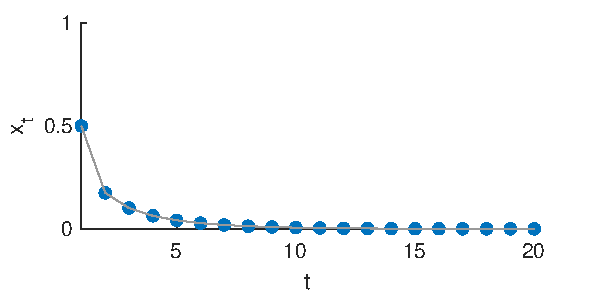
\includegraphics[width=8cm]{figures/ch3/logistic_map.pdf}
\caption{Example for the evolution of the logistic map with $k = 0.7$ and $x_1 = 0.5$.}
\label{fig:logistic_map}

\end{figure}

Depending on how the growth rate is chosen, the system can exhibit a variety of patterns. Figure \ref{fig:more_logistic_maps} gives examples for the logistic map with different values for the growth rate $k$. In all cases, $x_1$, the initial state, is $0.42$. In the case of $k = 1.2$ (top left), the system monotonically approaches one value. This type of attractor is called \emph{point attractor}, it is the same kind of attractor as the one in the illustration of Figure \ref{fig:logistic_map}. In the case of $k = 2.9$ (top right), the system also approaches one steady state, but while approaching the attractor, it alternates from one side to the other. When $k = 3.3$ (bottom left), the attractor of the system is not a steady state. Instead, the system oscillates between two values. This is type of attractor is called a \emph{limit cycle}. Another interesting case is $k = 4$ in which the system also oscillates but not in a periodic manner. This behaviour is called \emph{chaos} \citep{KaplanGlass1995}. When exhibiting chaotic behaviour, the system will never settle in a steady state or limit cycle but oscillate forever without repeating itself. 

\begin{figure}
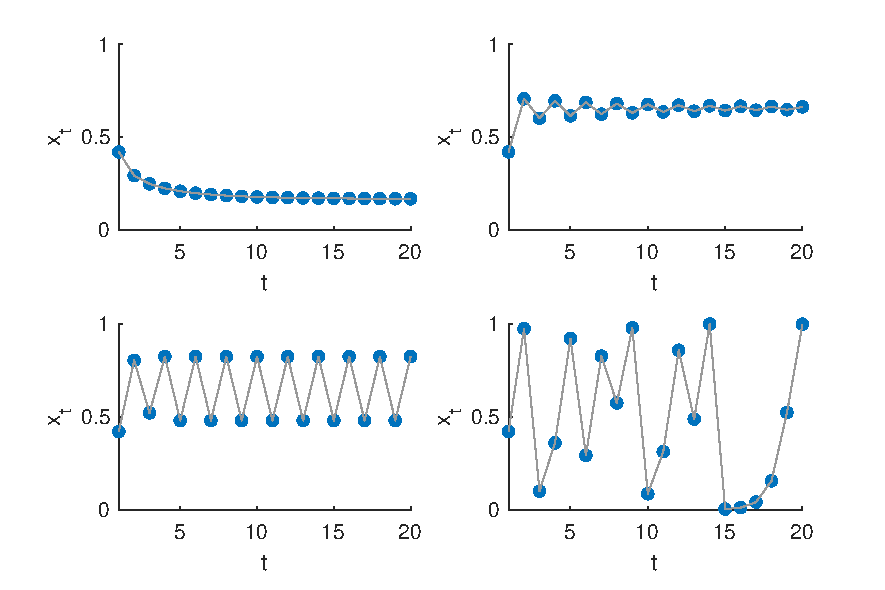
\includegraphics[width=\textwidth]{figures/ch3/more_logistic_maps.pdf}
\caption[Example for the evolution of the logistic map with different values for the growth parameter.]{Example for the evolution of the logistic map with different values for the growth parameter (top left: $k = 1.2$, top right: $k = 2.9$, bottom left: $k = 3.3$, bottom right: $k = 4$).}
\label{fig:more_logistic_maps}
\end{figure}

Figure \ref{fig:logistic_map_bifurcation} illustrates the possible patterns of the logistic map as the growth parameter is changed. The plot, also known as a \emph{bifurcation plot} \citep{Feigenbaum1978}, was created by running the logistic map for 2000 iterations for all growth parameter values between 1 and 4 with a step size of 0.01 (i.e. the simulation was first run with $k = 1$, then $k = 1.01$, then $k = 1.02$, and so on). The initial state is $0.42$ in all simulations. The axis for the parameter value is the x-axis. Of the 2000 iterations for each parameter value, the last 100 values are plotted on the y-axis as single tiny dots. For $k < 3$, all dots are plotted on top of each other because after a few iterations the system reached a steady state. As the parameter $k$ is increased, the system’s attractor is a limit cycle that oscillates between two values. The cycle frequency is then increased to 4, 8, 16 until the system eventually exhibits aperiodic behaviour as described above. There are, however, bands of growth parameter values in between for which the system moves back to periodic cycles (visible as white stripes in the higher regions on the x-axis) \citep{KaplanGlass1995, Spivey2007}. The behaviour of the system as $k$ is scaled beyond 3.5 can be observed in more detail in Figure \ref{fig:logistic_map_bifurcation_zoom}. This figure shows the same plot as Figure \ref{fig:logistic_map_bifurcation} with the x-axis zoomed in to the range of $k$ values from 3.5 to 4.

\begin{figure}
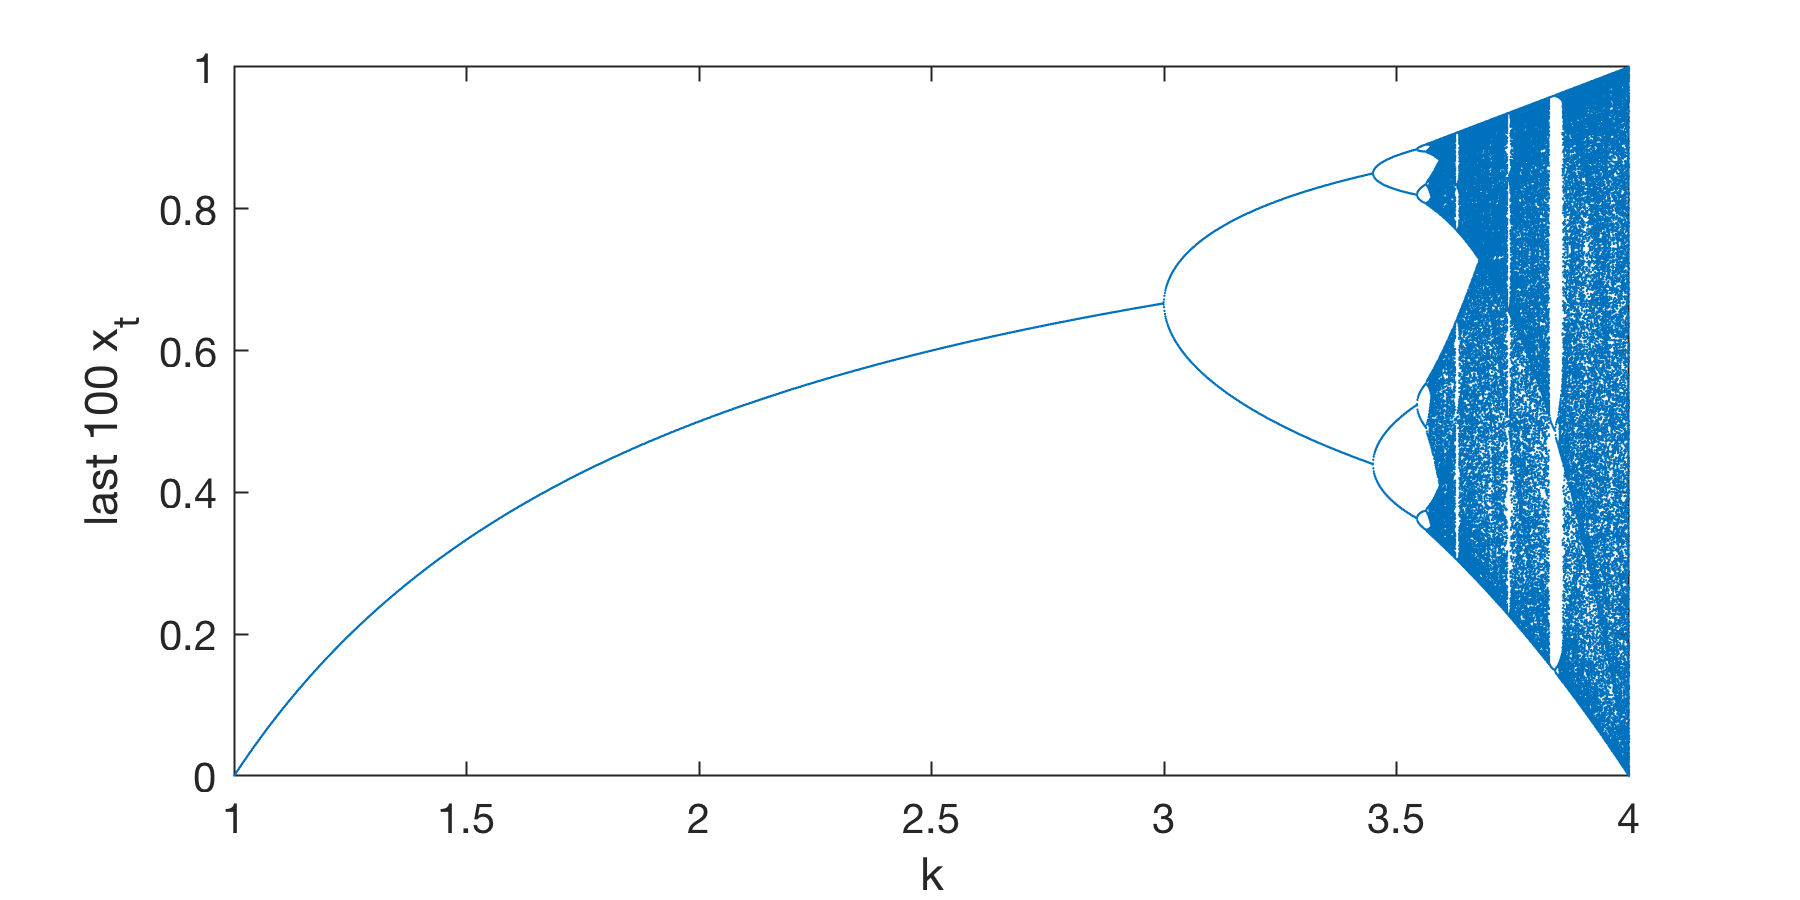
\includegraphics[width=\textwidth]{figures/ch3/logistic_map_bifurcation.png}
\caption{Bifurcation plot of the logistic map.}
\label{fig:logistic_map_bifurcation}
\end{figure}

\begin{figure}
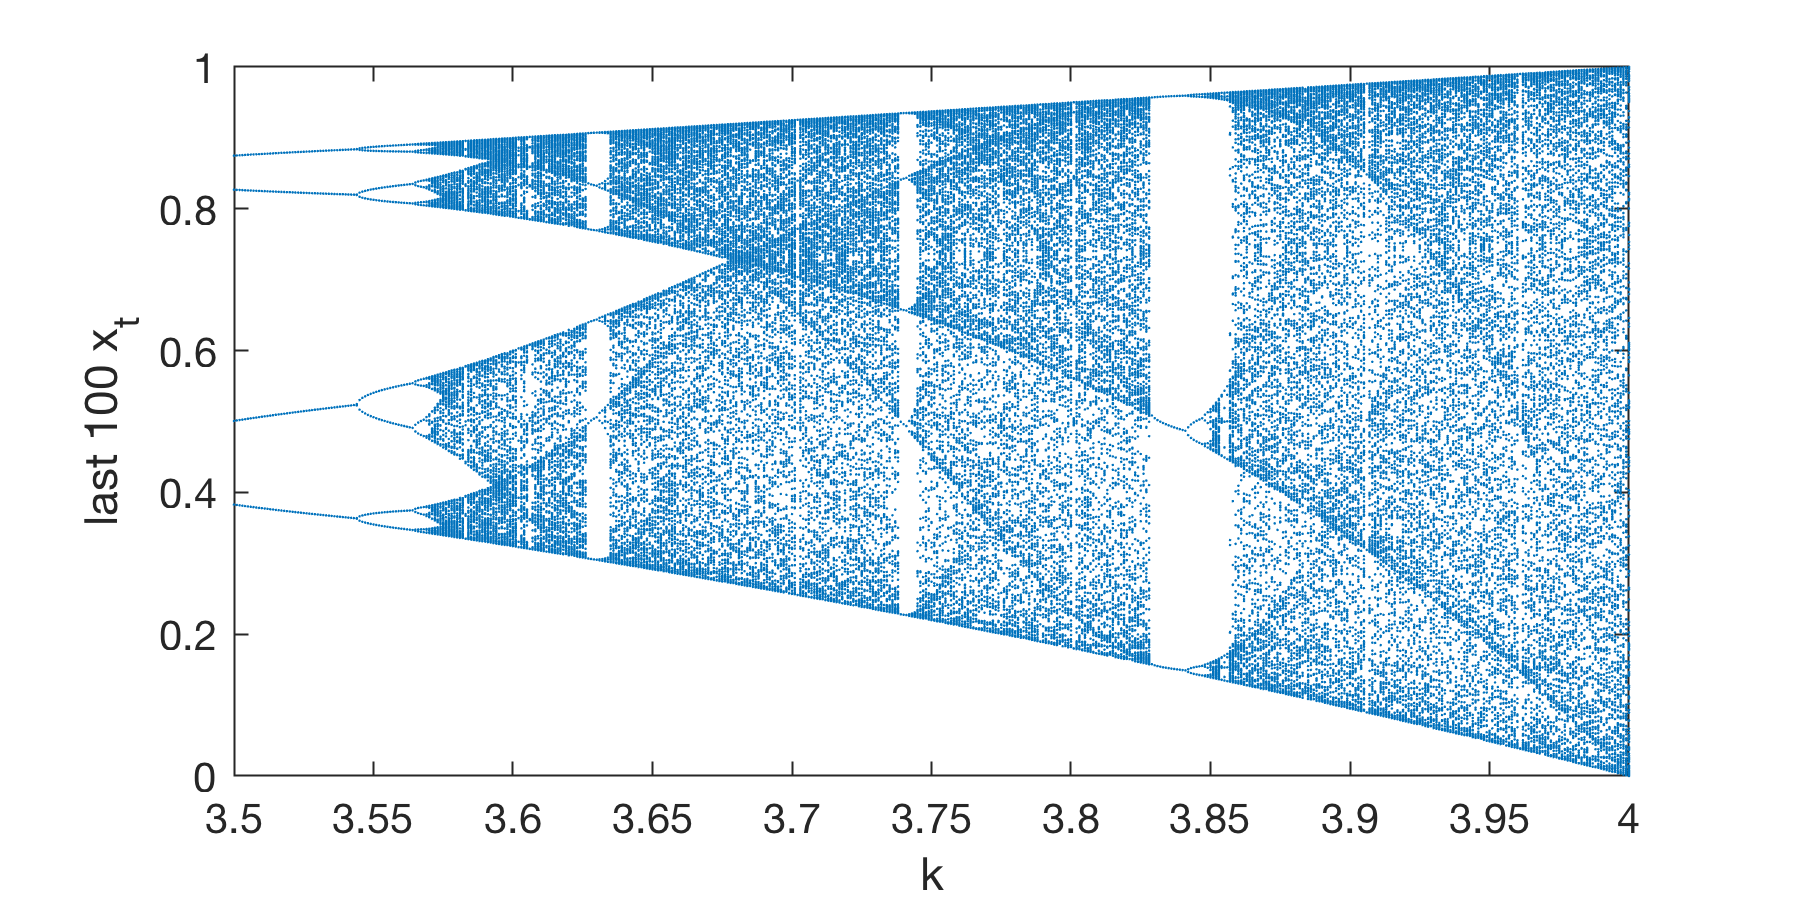
\includegraphics[width=\textwidth]{figures/ch3/logistic_map_bifurcation_zoom.png}
\caption{Bifurcation plot of the logistic map for values of $k \geq 3.5$.}
\label{fig:logistic_map_bifurcation_zoom}
\end{figure}

The examples presented around the logistic map demonstrate that an attractor can be a single value or a set of values. For the present work, point attractors will be most important. To change the behaviour of the system, the examples adjusted the growth parameter value $k$. A parameter like $k$ is called a \emph{control parameter} -- a very important concept for the understanding of dynamical systems. Control parameters can be thought of as the parameters that ``move the system through its repertoire of patterns and cause them to change" \citep[1538]{Kelso2013}. They often represent environmental conditions, like the growth parameter in the logistic map example, but are not restricted to this role \citep{Kelso2013}. 

An essential property of dynamical systems is that they often exhibit \emph{qualitative change} as the control parameter is scaled. This behaviour is referred to as \emph{bifurcation} -- a term used above already with regard to Figure \ref{fig:logistic_map_bifurcation} and \ref{fig:logistic_map_bifurcation_zoom}. As the name of the chart displayed in the two figures, bifurcation plot, already suggested, it shows how the logistic map undergoes bifurcation as the control parameter (the growth parameter) is increased. While the system starts with a point attractor, it changes into a pattern with a limit cycle as the control parameter passes a critical threshold. Subsequently, for other control parameter thresholds, the periods of the cycles change before the system turns to aperiodic behaviour. It then changes between aperiodic and periodic patterns for different ranges of control parameter values. All these transitions are qualitative changes, i.e. bifurcations, in the dynamical system.

\medskip\noindent \textit{Code used in this section: logistic\_map\_evolution.m, logistic\_map\_bifurcation.m}

\subsection{The use of differential equations in dynamical systems}
\label{sec:diff_equations}

In the logistic map, time progresses in discrete steps (or generations). When solving the equation, one considers the time points $t_1, t_2, t_3, ..., t_n$. In reality, of course, time is best characterised as continuous. A very common way to describe a dynamical system with reference to continuous time is by using \emph{differential equations}. The equation in \ref{eq:straight_line} gives a simple example for a differential equation. It uses a very common notation with a dot above the $x$ which denotes that the function is a derivate with respect to time, $\dot{x} = \frac{dx}{dt}$ \citep{Fuchs2013}. The basic idea in this system is very similar to the logistic map: We observe the behaviour of the state variable $x$. To learn about the change of the system at each state of $x$, the differential equation of the system is solved.

\begin{equation}
\dot{x} = kx
\label{eq:straight_line}
\end{equation}

To get an impression of what this simple system does, it is useful to start at some randomly chosen state and look at the evolution of the state variable $x$ over time. One way is to use a method known as the \emph{Euler method}, named after Swiss mathematician Leonhard Euler.\footnote{There are also other methods to solve differential equations, like the Runge-Kutta method. For some systems, like the one of Equation \ref{eq:straight_line}, it is also possible to give an exact analytical solution. For the exposition of systems considered in this work, subtle differences between the methods do not play a role.} Simply speaking, this method takes the change at the current state -- calculated by solving the differential equation of the system -- and adds it to the current state. Given that the state at some time point $t$ is known, the state at time point $t+h$ can be calculated easily as $x_t + hkx_t$ \citep{Fuchs2013} where $h$ denotes the size of the step that is taken in time (also expressed as $\Delta t$). As noted above, time is conceptualised as continuous in differential equations with regard to time, so using a discretising solution seems somehow paradoxical. However, it provides an easily implemented computation method for the solution of differential equations and the step size $h$ can be chosen very small to account for the fact that in continuous time the difference between $t$ and $t+1$ converges to zero. For the present work, the approximation of continuous time with sufficiently small time steps will be accepted as it will not disturb the results of the account. Figure \ref{fig:evolution_of_straight_line1} presents the evolution of the system of \ref{eq:straight_line} with a $k$ of $-0.5$ starting at the initial state $x = 0.42$. Similar to the example of \ref{fig:logistic_map}, this system approaches an attractor at zero.

\begin{figure}
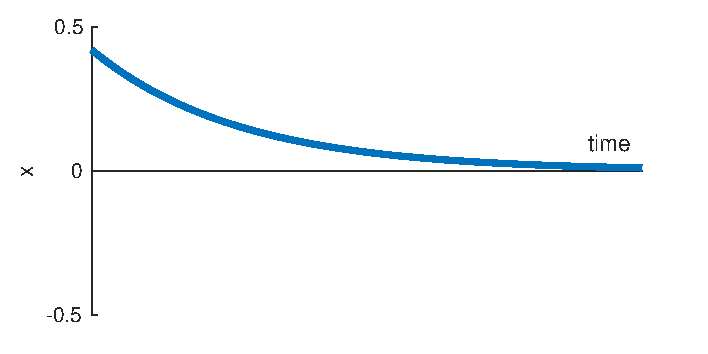
\includegraphics[width=9.5cm]{figures/ch3/evolution_of_straight_line1.pdf}
\caption{Evolution of the system given by the differential equation $\dot{x} = kx$ for $k = -0.5$.}
\label{fig:evolution_of_straight_line1}
\end{figure}

Figure \ref{fig:evolution_of_straight_line2} demonstrates the effect of scaling the control parameter. For all values of $k$, the system stays at zero if the initial state is zero (yellow lines). This is because the change in the system is given by $\dot{x} = kx$ and if $x$ is zero, the change will be zero as well. For all other initial values, the following pattern can be observed: $k$ values smaller than zero make the system approach the attractor at zero. For k values greater than zero, the system does not converge to any attractor. With $k = 0$ the system does not change at all but stays in its initial state. 

\begin{figure}
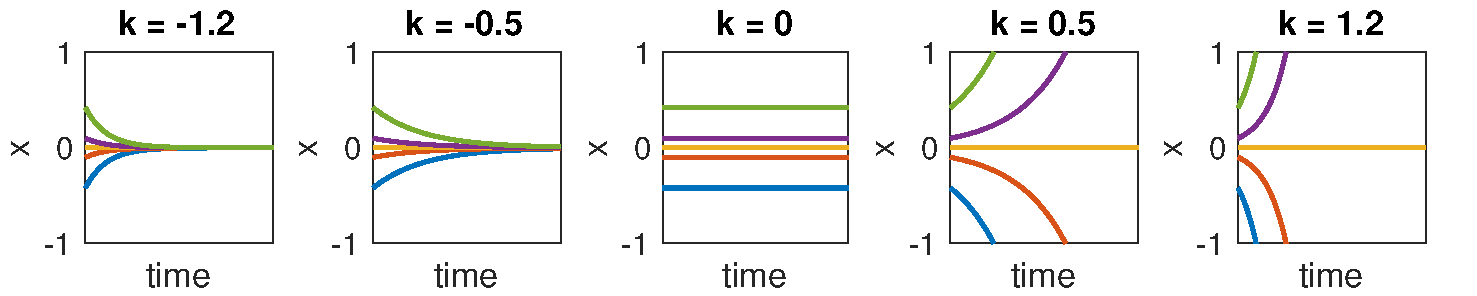
\includegraphics[width=\textwidth]{figures/ch3/evolution_of_straight_line2.pdf}
\caption[Evolution of the system given by the differential equation $\dot{x} = kx$ for different values of the control parameter $k$.]{Evolution of the system given by the differential equation $\dot{x} = kx$ for different values of the control parameter $k$. Colours indicate initial states: green = $0.42$, purple = $0.1$, yellow = $0$, red = $-0.1$, blue = $-0.42$.}
\label{fig:evolution_of_straight_line2}
\end{figure}

To learn about the patterns of the system without calculating solutions, a \emph{phase space plot} can be a useful tool \citep{Fuchs2013}. In a phase space plot it is particularly interesting to look for \emph{fixed points} -- points where the differential equation is zero, i.e. $\dot{x} = 0$. Figure \ref{fig:phase_space_straight_line} shows the phase space plots for $\dot{x} = kx$, for $k<0$ and $k>0$. The solutions for the system showed that nothing happens when $k = 0$, the system remains in its initial state. Hence, this case will not be discussed any further here and it will only be investigated what happens for $k < 0$ and $k > 0$. First, the left plot of Figure \ref{fig:phase_space_straight_line} is discussed where the control parameter $k$ is below zero. The function $\dot{x}$ has positive values for negative $x$ values, and negative values for positive $x$ values. Whenever the system is in a negative state (negative $x$), the change given by $\dot{x}$ is positive, so the system moves towards zero from the left side. Whenever the system is in a positive state (positive $x$), the change given by $\dot{x}$ is negative, so the system moves towards zero from the right side. This direction is indicated by the arrows on the x-axis. The further away the value of $x$ from zero, the greater the change -- this is shown by the size of the arrows. In addition, it is clear that $\dot{x} = 0$ for $x=0$. In sum, for $k<0$, when the system is at zero, it stays there; when it is in some other state (be it negative or positive), it gravitates towards zero. The black filled circle at zero indicates that zero is a \emph{stable fixed point} of the system, an attractor. 

\begin{figure}
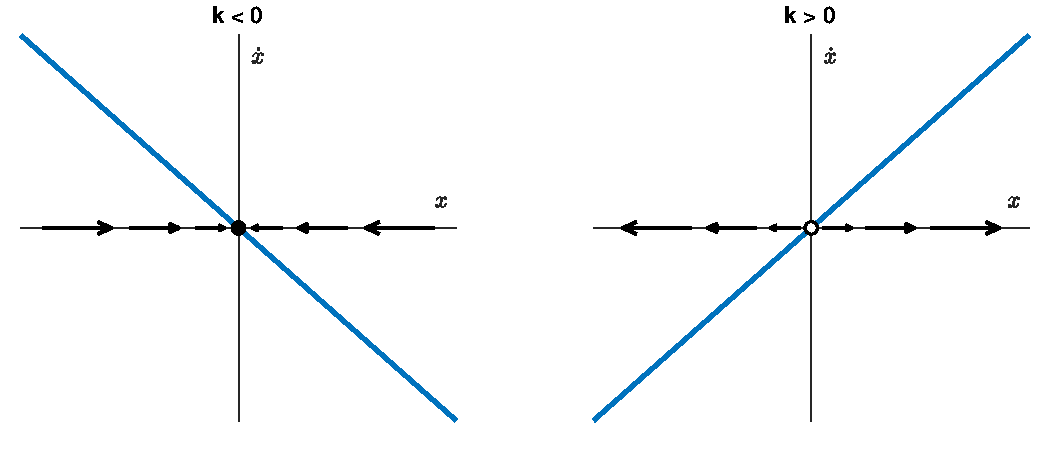
\includegraphics[width=\textwidth]{figures/ch3/straight_line.pdf}
\caption[Phase space plot of $\dot{x} = kx$.]{Phase space plot of $\dot{x} = kx$. Arrows indicate the direction of change in the system. The filled circle stands for attractor, the empty circle stands for repeller.}
\label{fig:phase_space_straight_line}
\end{figure}

In the right plot, the space phase plot is shown for cases in which the control parameter $k$ is greater than zero. Whenever the system is in a negative state (negative $x$), the change given by $\dot{x}$ is negative, so the system moves further away from zero towards $-\infty$. Whenever the system is in a positive state (positive $x$), the change given by $\dot{x}$ is positive, so the system moves further away from zero towards $\infty$. When the system starts at $x = 0$, it will stay there. But this is the only possibility to be in the state of zero for $k > 0$. All other initial states will lead away from zero, even states that are very close to zero, as for example $x = \frac{1}{10000}$. This is again indicated by the arrows, in this case pointing away from zero. Zero in this scenario is called an \emph{unstable fixed point} or \emph{repeller}, represented by an empty circle.

\medskip\noindent \textit{Code used in this section: ds\_straight\_line.m}

\subsection{Multistability}

Dynamical systems can have more than one attractor -- a situation called \emph{multistability}. Multistability is different to the ranges of control parameter values in the logistic map that exhibit a limit cycle attractor. In the case of the limit cycle, all values in the set of the attractor will be visited – the system oscillates between these values. The whole set is one attractor. In the case of a system with more than one attractor, the initial state is crucial in determining in which of the attractors the system will settle. At the end of this chapter, the concept of the stochastic dynamical system will be presented. In this case, random fluctuations play an important part and the role of the initial state in a multistable system is diminished.

The system that will be used here to illustrate the situation in which more than one attractor is present is the one defined by the differential equation in \ref{eq:double_well_force}, a system that will play a major role in this work. Figure \ref{fig:double_well_evolution} gives the solutions for some values of $k$ and some intitial states. Two aspects are important here: First, for $k = 0$ and $k = \pm0.2$, some trajectories settle in a positive attractor, others settle in a negative attractor. The attractor in which the system settles depends on the initial state. Second, for $k = \pm0.7$, the situation is different, the system only settles in one attractor regardless of the initial state.

\begin{equation}
\dot{x} = k + x - x^3
\label{eq:double_well_force}
\end{equation}

\begin{figure}
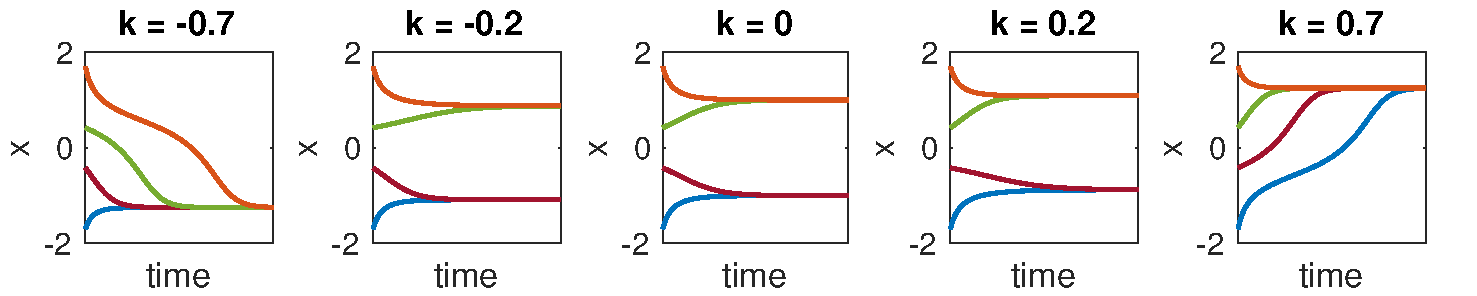
\includegraphics[width=\textwidth]{figures/ch3/evolution_of_double_well.pdf}
\caption[Evolution of the system given by the differential equation $\dot{x} = k + x - x^3$ with different control parameter $k$ values and different initial conditions.]{Evolution of the system given by the differential equation $\dot{x} = k + x - x^3$ with different control parameter $k$ values and different initial conditions. Colours indicate initial states: blue = $-1.7$; red = $-0.42$; green = $0.42$; orange = $1.7$.
}
\label{fig:double_well_evolution}
\end{figure}

The behaviour of this system can again be illustrated by the phase space plots \citep{Fuchs2013}, see Figure \ref{fig:double_well_force}. As before, an attractor is drawn as a full circle, a repeller is drawn as an empty circle. When the control parameter is zero, i.e. $k = 0$ (plot in the centre), two attractors and a repeller in the middle exist. When the control parameter is decreased (top row) or increased (bottom row), the attractor layout first remains as described until critical thresholds of the control parameter on both sides (increasing and decreasing) are reached. The symbols $-k_c$ and $+k_c$ stand for these critical values of the control parameter. When $k$ is smaller than $-k_c$, only one attractor exists, and this attractor is located in the negative range of the state axis. When $k$ greater than $k_c$, only one attractor exists in the system, and this attractor is located in the positive range of the state axis. 

When $k$ equals $-k_c$ or $k_c$, a \emph{half stable point} exists on the opposite side of the attractor, drawn as a square. This point acts like an attractor from one side but like a repeller from the other side. For example, when $k = -k_c$ (second plot in top row), the system will settle in this point when starting with an initial value that is greater than the location of this half stable point, i.e. coming from far right on the x-axis. On the contrary, when the initial state is a tiny bit to the left of the half stable point, the system will converge towards the attractor in the negative range on the x-axis.

In sum, this system exhibits bistability -- the presence of two attractors -- when $k$ is in the range between $-k_c$ and $k_c$ (i.e. $-k_c < k < k_c$). When the control parameter reaches the critical value on one or the other side ($-k_c$ or $k_c$), bifurcation occurs and the bistability breaks down: One attractor turns into a half-stable point at the respective critical threshold; beyond the critical values, even this half-stable point vanishes.

\begin{figure}
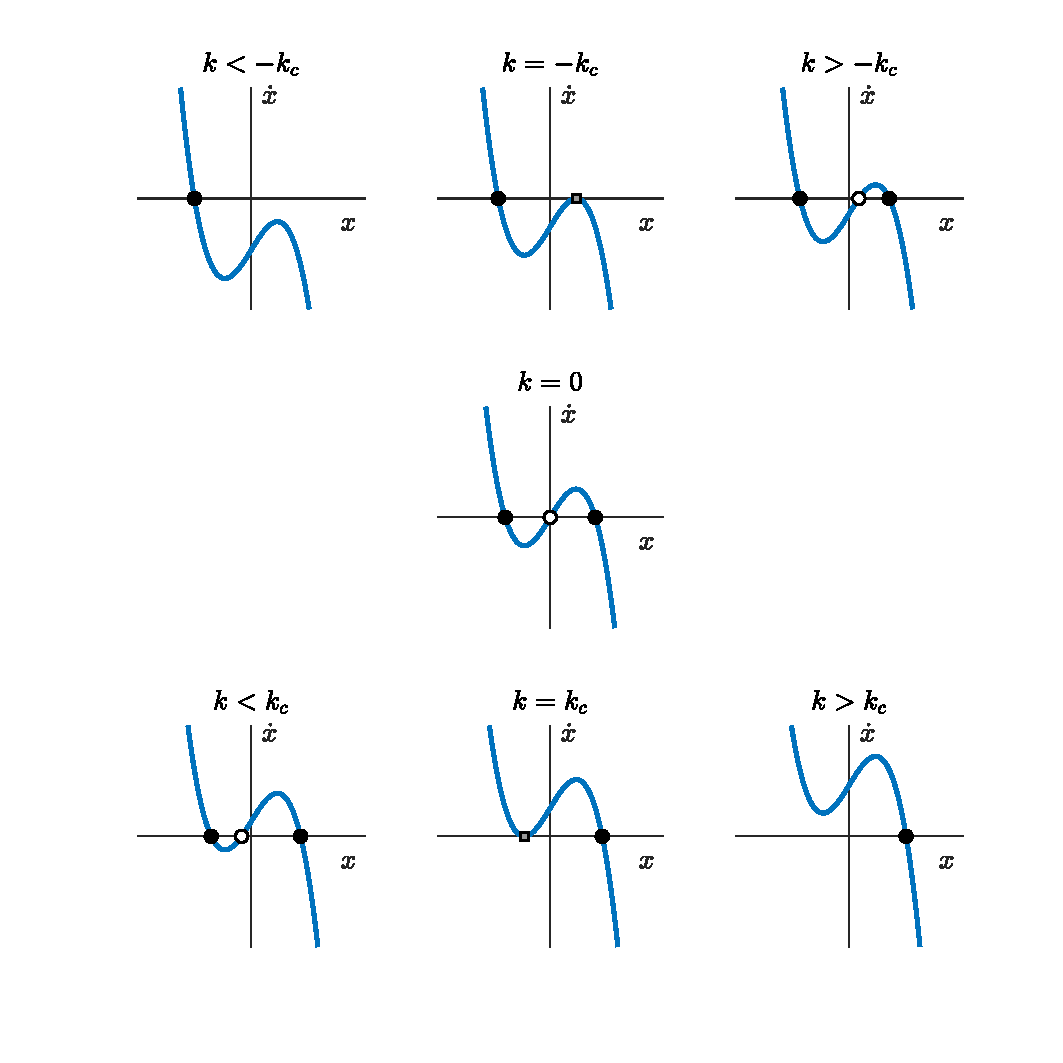
\includegraphics[width=\textwidth]{figures/ch3/double_well_force.pdf}
\caption[Phase space plot for $\dot{x} = k + x - x^3$.]{Phase space plot for $\dot{x} = k + x - x^3$. The filled circle stands for an attractor, the empty circle stands for a repeller, the square stands for a half-stable point.}
\label{fig:double_well_force}
\end{figure}

So far, differential equations have been used to represent a dynamical system. An additional, tightly connected way to define a dynamical system is by its \emph{potential function}. The potential is given by the negative integral of the differential equation. Thus, the relation of the differential equation, which is also often called the \emph{force function}, and the potential can be expressed as $\dot{x} = F(x) = -\frac{dV(x)}{dx}$, where $V(x)$ is the potential and $F(x)$ is the force. The graph of the potential function visualises the \emph{attractor landscape} of the dynamical system. Attractors appear as ``valleys", i.e. local minima in the graph. Figure \ref{fig:double_well_potential} gives the potential for the system defined by its differential in Equation \ref{eq:double_well_force}, the potential function itself is given in Equation \ref{eq:double_well_potential}. A commonly used metaphor for making the behaviour of the system understandable more intuitively is to imagine a ball or a marble rolling through the attractor landscape given by the potential \citep{HakenLevi2012}, since ``[t]he temporal evolution of a one-dimensional dynamical system corresponds to an overdamped motion of a particle in the landscape of its potential" \citep[22]{Fuchs2013}. Crucially, one has to think of the motion of the ball in ``thick or viscous fluid like honey" such that when ``it reaches a minimum it will stick there and will not oscillate back and forth" \citep[22]{Fuchs2013}.

\begin{equation}
V(x) = - kx - \frac{x^2}{2} + \frac{x^4}{4}
\label{eq:double_well_potential}
\end{equation}

Compare Figure \ref{fig:double_well_potential} (potential) to Figure \ref{fig:double_well_force} (force). When $k$ is zero, two symmetrical valleys are present in the potential. Because of this shape it is often called \emph{double-well potential}. Depending on where the ball starts, it rolls down either one of the valleys. When k is decreased or increased, the function tilts to one side, making one valley deeper and the opposite valley shallower. By passing the critical value of $k$ ($-k_c$ or $k_c$), one of the attractor valleys disappears -- in other words, the attractor becomes unstable and that state of the system ceases to be an attractor. Regardless of where the ball starts now, it will always roll into the remaining attractor. At the critical values, the ``fading attractor" takes an elbow shape. The ball metaphor can help to understand the fact that this point is half-stable: Suppose for instance that $k = -k_c$, if the ball starts on the right side of the half-stable point, it will roll down the potential to come to a halt at that point. If, on the contrary, it starts on the left side of the point, it will roll down to the attractor in the negative part of the x-axis. 

\medskip\noindent \textit{Code used in this section: double\_well.m}

\begin{figure}
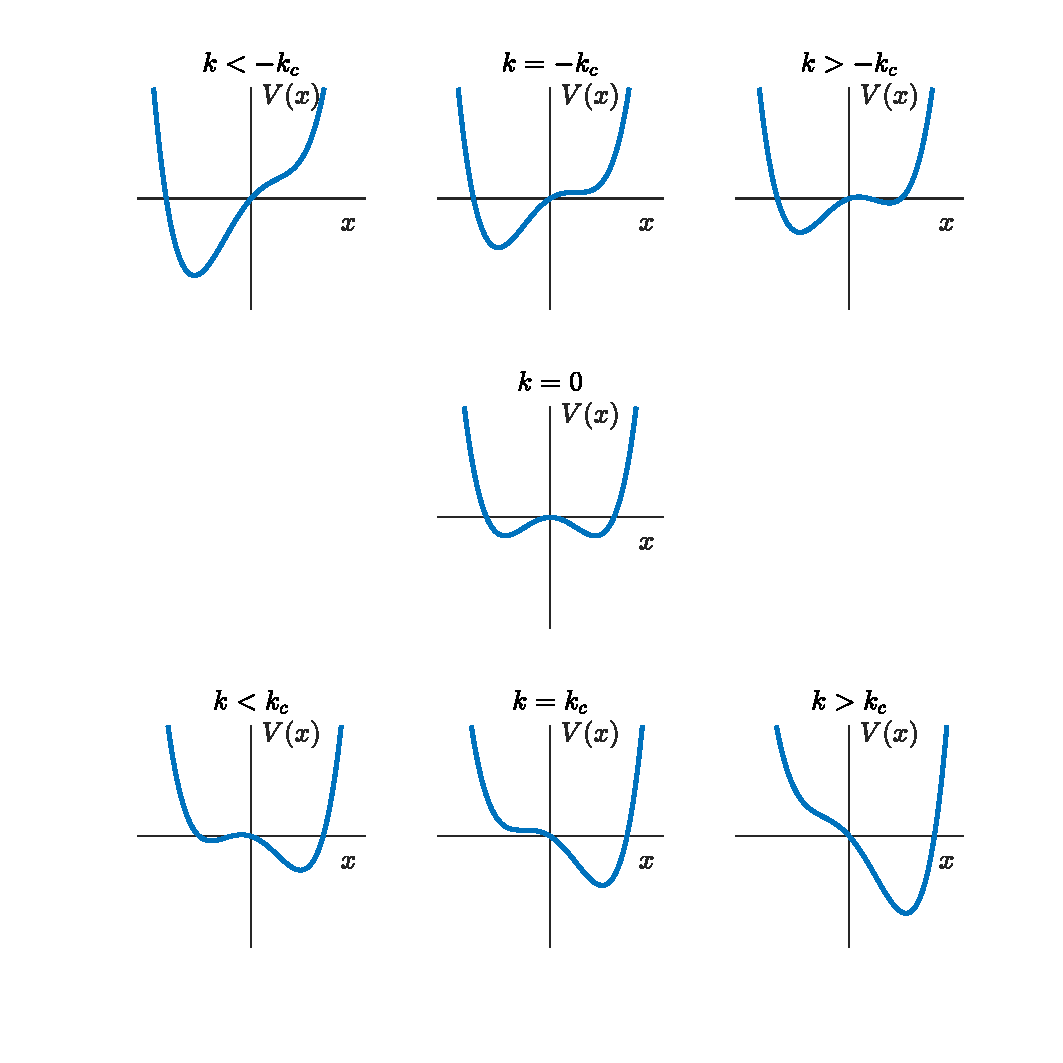
\includegraphics[width=\textwidth]{figures/ch3/double_well_potential.pdf}
\caption{Potential $V(x) = - kx - \frac{x^2}{2} + \frac{x^4}{4}$ corresponding to the phase space plots of the force $\dot{x} = k + x - x^3$.}
\label{fig:double_well_potential}
\end{figure}

\section{Applications of dynamical systems}

This chapter so far has outlined some of the basics of dynamical systems. In what follows, applications in the realm of human movement, language and speech will be discussed. This section presents a non-exhaustive collection of applications. The models are explained in some detail as they provide inspiration for the modelling approach presented in the second part of the book.

\subsection{Modelling coordination and speech dynamics}

Patterns of human motion have been fruitfully described in terms of dynamical systems. Since speech production represents a highly intricate system of coordinated movements, a large and growing body of research has applied nonlinear dynamics to speech. The present subsection introduces and highlights some interesting points of this research.

\subsubsection{Inter-limb coordination}

An influential application of dynamical systems in the domain of human behaviour is the model of \citet{HakenKelsoBunz1985}. This model presents a mathematical description of interesting observations on the coordination patterns of finger movements made in earlier research by one of the authors. In the study of \citet{Kelso1981}, the subjects moved the index fingers of both hands simultaneously at varying frequencies. One remarkable finding was that subjects were able to coordinate the movements of their fingers in two different stable modes: anti-symmetrically, a coordination pattern also known as \emph{anti-phase}, or symmetrically, a coordination pattern known as \emph{in-phase}. These two modes are illustrated in Figure \ref{fig:hkb_fingers}.

\begin{figure}
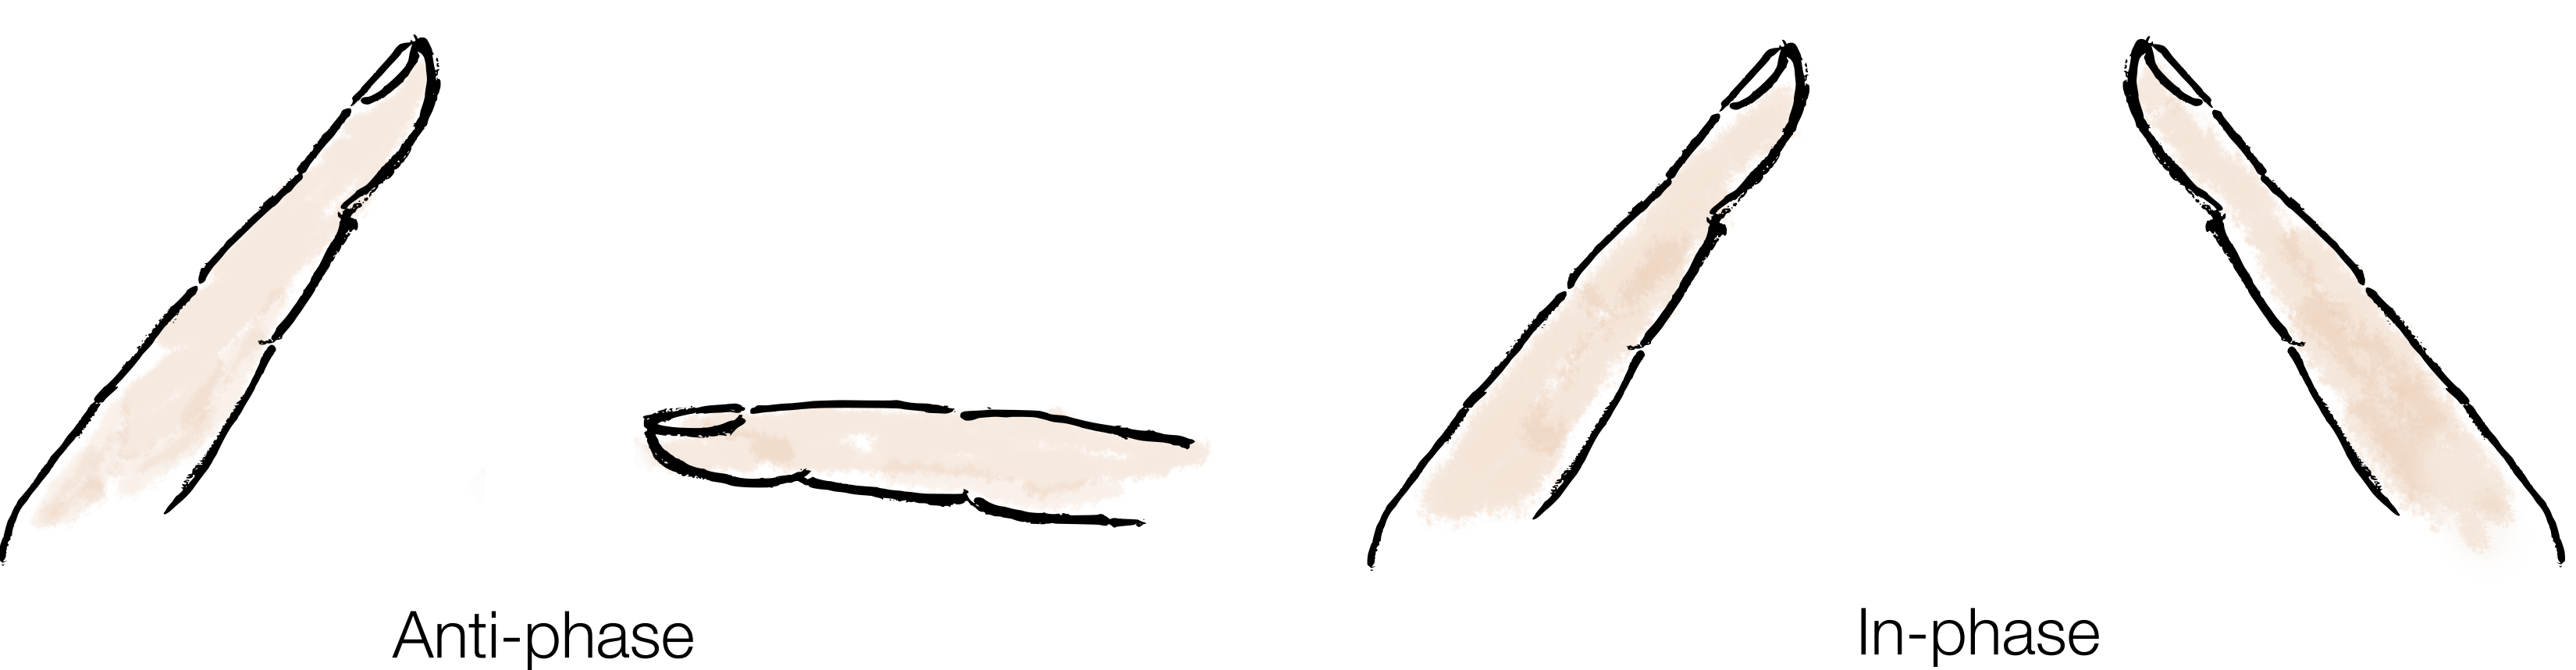
\includegraphics[width=11cm]{figures/ch3/hkb_fingers.png}
\caption[Stable coordination patterns found in \citet{Kelso1981}.]{Stable coordination patterns found in \citet{Kelso1981} and used for the modelling approach in \citet{HakenKelsoBunz1985}: anti-phase vs. in-phase.}
\label{fig:hkb_fingers}
\end{figure}

In terms of a dynamical model, the movement of each finger can be idealised as a harmonic oscillation and each oscillation can be described by its phase angle $\phi_i$ \citep{HakenKelsoBunz1985}. When modelling the coordination patterns introduced in the last paragraph, the \emph{relative phase} is of primary concern. Let $\phi_1$ and $\phi_2$ be the phase angles of the respective fingers, then $\phi = \phi_2 - \phi_1$ is the relative phase. In the right panel of Figure \ref{fig:hkb_phase_position}, the oscillations of the two fingers in anti-phase (top) and in-phase (bottom) are shown.\footnote{The oscillations for both fingers have identical frequencies and amplitudes in this example.} The dashed line marks one time point $t_1$. The left panel gives the phase angles of the oscillations at this time point $t_1$. When the oscillations of the fingers are in anti-phase mode (top), the phase angles are displaced by 180°, i.e. the relative phase $\phi$ is 180°. At $t_1$, $\phi_1$ is 40° and $\phi_2$ is 220° and consequently $\phi=\phi_2-\phi_1=180$°. The relative phase is visualised by the grey shaded circular sector in the phase angle plot on the left. When the oscillations of the fingers are in in-phase mode (bottom), their phase angles are identical and the relative phase is 0°. At $t_1$ in the lower panel, both $\phi_1$ and $\phi_2$ are 220°, hence $\phi = \phi_2 - \phi_1 = 0$°. When plotted on top of each other, only one of the oscillations is visible in this case. 

\begin{figure}
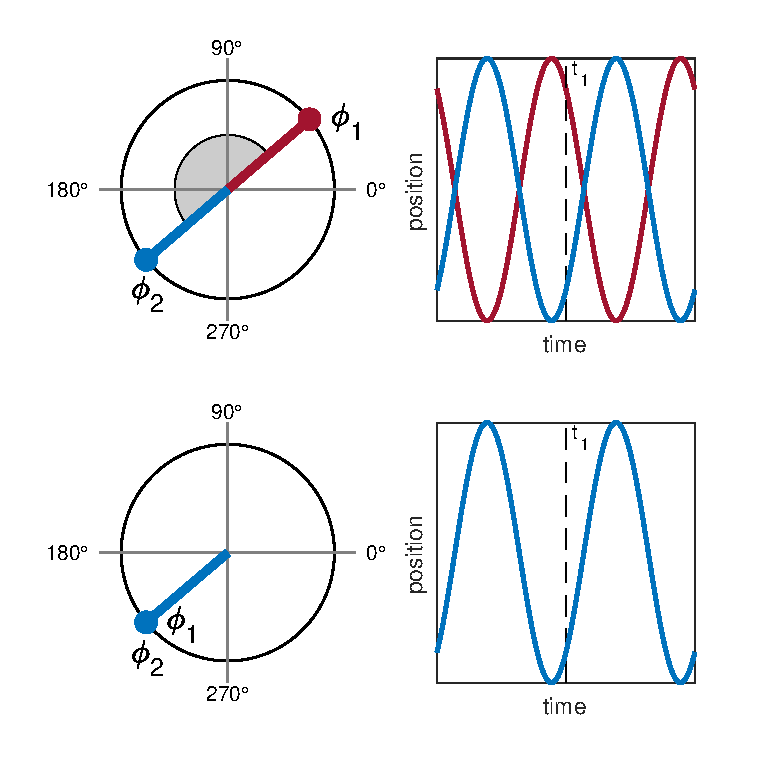
\includegraphics[width=10cm]{figures/ch3/phase_position_hkb_fingers.pdf}
\caption{Phase angles and evolution of the oscillatory finger movements as modelled by \citet{HakenKelsoBunz1985}.}
\label{fig:hkb_phase_position}
\end{figure}

An additional result of \citet{Kelso1981} was that when subjects started to move their index fingers in anti-phase (as in the top panel of \ref{fig:hkb_phase_position}) and the frequency of this movement was increased, the subjects' finger movements changed abruptly to an in-phase coordination (as in the bottom panel of \ref{fig:hkb_phase_position}) at a critical frequency boundary. To capture these findings, \citet{HakenKelsoBunz1985} proposed a model that has attractors for anti-phase and in-phase coordination for certain ranges of the control parameter and a single attractor for in-phase coordination when the control parameter is scaled past a critical threshold. The model is given by its potential energy function in Equation \ref{eq:hkb_potential}. The control parameter is the ratio of $b$ and $a$, i.e $\frac{b}{a}$. The potential is in fact periodic and so the shape of the attractor landscape repeats over and over again with $V(\phi + 2\pi) = V(\phi)$. 

\begin{equation}
V(\phi) = -a \cos(\phi) - b \cos( 2 \phi)
\label{eq:hkb_potential}
\end{equation}

In the model, increasing frequency of the movements is conceptualised as a decrease in the ratio $\frac{b}{a}$. Figure \ref{fig:hkb_landscapes} illustrates the attractor landscapes for different values of the $\frac{b}{a}$. To interpret the effect of scaling $\frac{b}{a}$ towards zero, the metaphor of a ball rolling down the attractor landscape can be employed again. In the figure, the ball starts in one of the anti-phase attractors with $\frac{b}{a} = 1$ (top left). This attractor is at $\phi = \pi$ which is the phase angle of 180° in radians. When going from left to right and top to bottom in the plot, the tempo of the finger movement increases and the ratio $\frac{b}{a}$ decreases. However, at first, the ball stays in the initial anti-phase attractor. This attractor basin becomes shallower until it is not an attractor basin anymore. At this critical value of $\frac{b}{a}$ (see lower left corner), the ball will be set into motion and roll down to the in-phase attractor which is at $\phi = 0$.

\begin{figure}
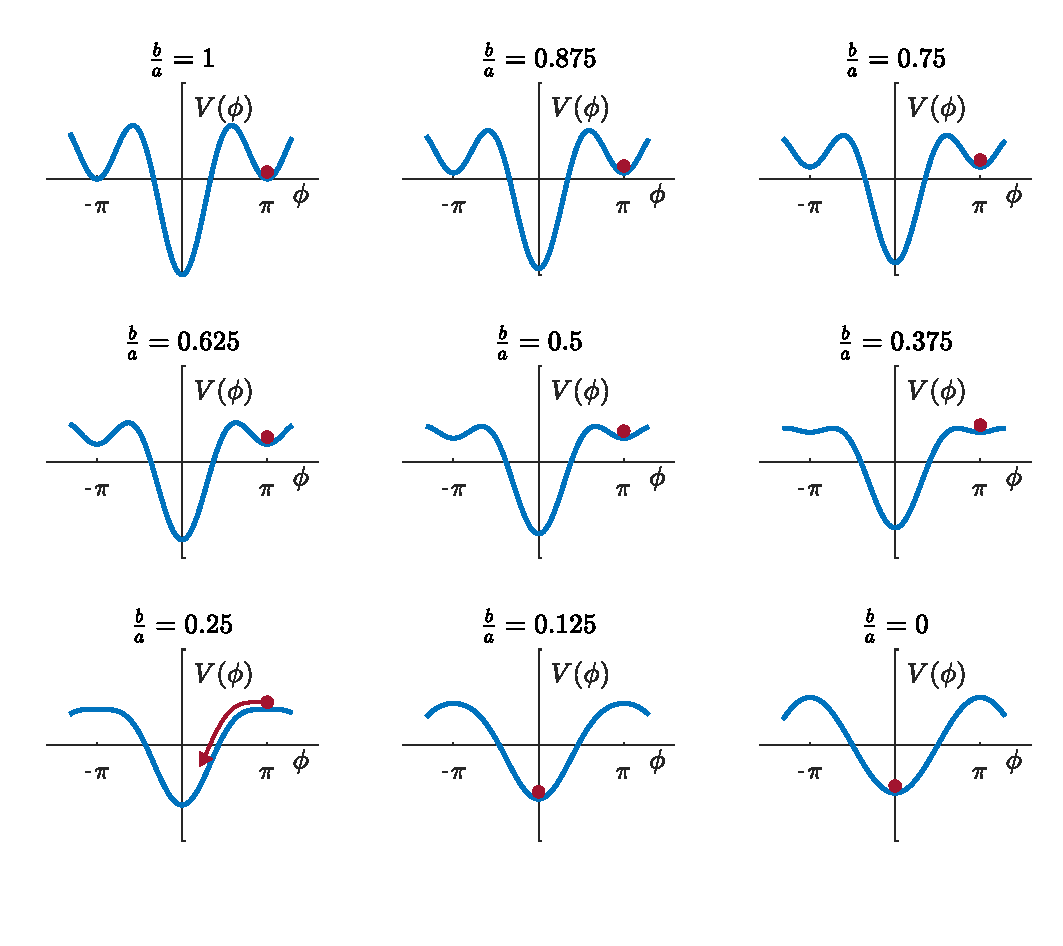
\includegraphics[width=\textwidth]{figures/ch3/hkb_potential.pdf}
\caption{Attractor landscapes of \citet{HakenKelsoBunz1985} for different values of $\frac{b}{a}$.}
\label{fig:hkb_landscapes}

\end{figure}

Figure \ref{fig:hkb_simulation} shows what happens to the oscillatory finger movements (upper pannel)  and their relative phase (middle panel) over time when the ratio $\frac{b}{a}$ drops beyond the critical value. As can be seen in the middle panel, the relative phase changes from anti-phase to in-phase abruptly -- with a small portion of instability after which the oscillations of the fingers in the top panel are exactly synchronous (and thus plotted on top of each other).

Hence, this dynamical model that is able to account for two qualitatively distinct coordination modes of finger motion using a potential function that is modulated by scaling a continuous parameter (or the ratio of two parameters). The model was in fact seminal and had great impact on models of speech production as will become clear in what follows. First, a closer look at the use of dynamics to model the \emph{gesture} in Articulatory phonology will be taken. Second, the coupled oscillator model for \emph{intergestural coordination} building upon \citet{HakenKelsoBunz1985} will be presented.

\begin{figure}
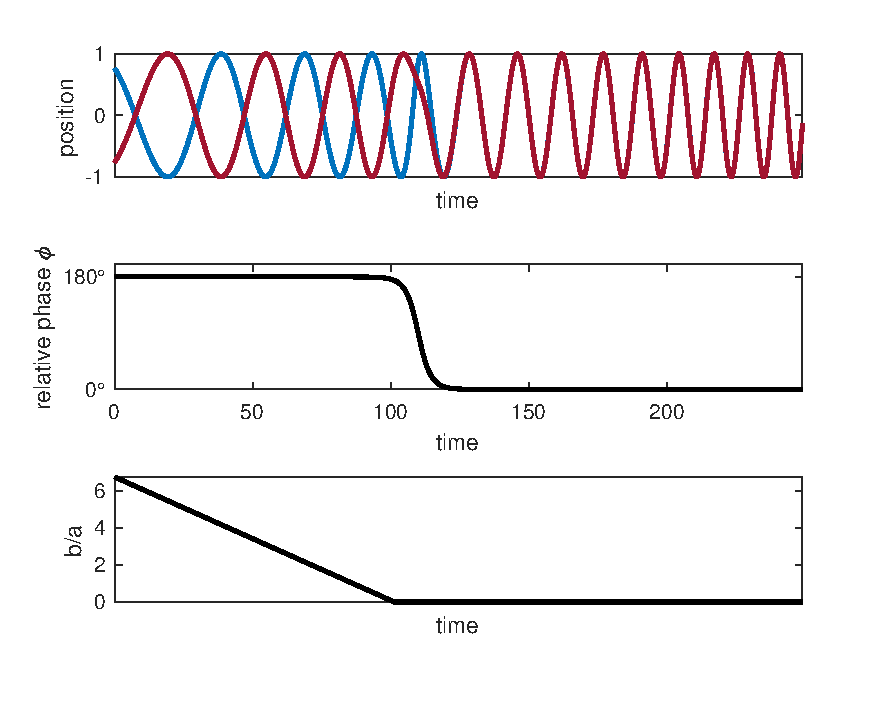
\includegraphics[width=12cm]{figures/ch3/hkb_simulation.pdf}
\caption{Simulation of the model of \citet{HakenKelsoBunz1985} starting in anti-phase mode and turning into in-phase mode.}
\label{fig:hkb_simulation}
\end{figure}

\medskip\noindent \textit{Code used in this section: hkb\_phase\_modes.m, hkb\_potential.m, hkb\_simulation.m}


\subsubsection{Articulatory gestures}

The framework of Articulatory phonology, as described in Chapter \ref{chapter_pandp}, views gestures as the primitives of phonology. Gestures are orchestrated to build higher forms like syllables and words. A gesture is defined in terms of a dynamical model. Chapter \ref{chapter_pandp} outlined how the model is able to account for variation in the speech signal, as for example the case of assimilation. In the current chapter, the model will be reviewed from the dynamical perspective.

Articulatory phonology builds upon a model known as \emph{task dynamics} to describe the gestures of speech production. Task dynamics (see \citealp{Saltzman1986, SaltzmanKelso1987, Saltzman1991}; as well as \citealp{Hawkins1992} for an introductory overview) has been developed to describe various patterns of movement that include multiple effectors like the shoulder, the upper and lower arm as well as the hand when grasping an object. Similar to other motion systems, speech involves the coordination of multiple effectors, in this case articulators, to form the relevant constrictions \citep{BrowmanGoldstein1989}. The task dynamics approach to articulation does not focus on the motion of the individual articulators but on the motion of \emph{tract variables} \citep{BrowmanGoldstein1992}. Tract variables describe the coordinative structures that jointly yield the relevant constrictions. For example, the upper lip, the lower lip and the jaw contribute to the tract variable of lip aperture \citep{BrowmanGoldstein1992}. Table \ref{tab:tract_vars} gives an overview of the tract variables and the articulators involved in these tract variables. Most tract variables come in “horizontal-vertical” pairs: Constriction location (horizontal) is combined with constriction degree (vertical). The gestures in Articulatory phonology are formed from the set of tract variables. When constriction degree and location are present, both dimensions are used to build the gesture.

\begin{table}
\caption{Tract variables of Articulatory phonology from \citet[73]{BrowmanGoldstein1989}.}
\begin{tabularx}{\textwidth}{Xll}
	\lsptoprule
&			\textbf{tract variable} &			\textbf{articulators involved}\\
\midrule
\textbf{LP} &		lip protrusion &				upper and lower lips, jaw\\
\textbf{LA} &		lip aperture &				upper and lower lips, jaw\\
\textbf{TTCL} &	tongue tip constriction location &	tongue tip, body, jaw \\
\textbf{TTCD} &	tongue tip constriction degree &		tongue tip, body, jaw \\
\textbf{TBCL} &	tongue body constriction location &	tongue body, jaw \\
\textbf{TBCD} &	tongue body constriction degree &	tongue body, jaw \\
\textbf{VEL} &	velic aperture &				velum \\
\textbf{GLO} &	glottal aperture &				glottis \\
  \lspbottomrule
\end{tabularx}
\label{tab:tract_vars}
\end{table}%

At the heart of the modelling approach of task dynamics is a dynamical system known as the \emph{damped harmonic oscillator} that specifies the control of a tract variable \citep{Hawkins1992}. It is formulated mathematically as the second order differential equation given in Equation \ref{eq:dho} \citep{SaltzmanKelso1987}. The systems reviewed in this chapter so far were given by first-order differential equations. In a second-order differential equation the second derivative, denoted by $\ddot{x}$, occurs.

\begin{equation}
m\ddot{x} + b\dot{x} + k(x-x_0) = 0
\label{eq:dho}
\end{equation}

The damped harmonic oscillator describes the motion of a mass attached to a spring that is stretched vertically \citep{FeynmanLeightonSands1963}, and is therefore often referred to as a spring-mass system. The state variable $x$ is the position of the mass attached to the spring, $\dot{x}$ is its velocity and $\ddot{x}$ is its acceleration. Besides $x$ and its two derivatives, a collection of parameters occurs in the equation: $m$, $b$, $k$ and $x_0$. These parameters are discussed shortly in this section; examples are given to illustrate the consequences of manipulating the parameters. 

The parameter $m$ refers to the mass attached to the spring. This parameter is usually set to 1 and not changed. For the sake of completeness, however, Figure \ref{fig:dho_mass}  shows what happens when the mass is changed (for this simulation, the parameter $b$ is set to 0, the parameter $k$ is set to 1, the parameter $x_0$ is set to 0). For higher values of $m$, the system oscillates at lower frequencies. It is easy to understand intuitively that greater masses need more time to be transported over the same distance compared to smaller masses. 

\begin{figure}[htp]
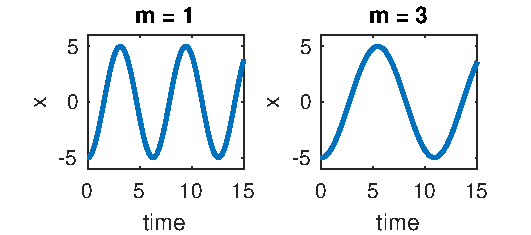
\includegraphics[width=7cm]{figures/ch3/dho_mass.pdf}
\caption{Consequences of scaling the parameter $m$ (mass) in the harmonic oscillator.}
\label{fig:dho_mass}
\end{figure}

The same effect is achieved by changing the parameter $k$, the stiffness of the spring, as shown in Figure \ref{fig:dho_stiff} (for this simulation, the parameter $b$ is set to 0, the parameter $m$ is set to 1, the parameter $x_0$ is set to 0). For higher values of $k$ the system oscillates at higher frequencies. Here as well, an intuitive understanding is facilitated by imagining the consequences of pulling two springs which differ with regard to their stiffness: The stiffer spring snaps back faster.

\begin{figure}
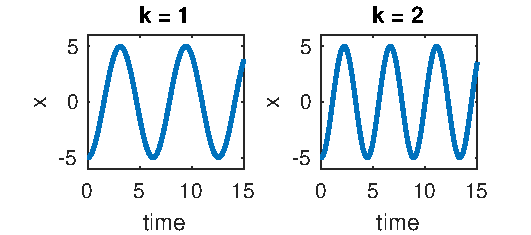
\includegraphics[width=7cm]{figures/ch3/dho_stiffness.pdf}
\caption{Consequences of scaling the parameter $k$ (stiffness) in the harmonic oscillator.}
\label{fig:dho_stiff}
\end{figure}

More important for the modelling of articulatory gestures is the parameter $b$, the damping of the system. Damping leads to dissipation of energy stored in the system due to friction and reduces (or even prevents) the system’s oscillation. Figure \ref{fig:dho_damp} illustrates four interesting cases of damping. In all cases, the mass $m$ and the stiffness $k$ are set to 1, $x_0$ is set to 0. In the top left plot, the undamped case is shown, $b = 0$. The system is \emph{not} damped, just like in the plots illustrating the changes of mass and stiffness. In this case, the system will oscillate forever. In the top right plot, the case of an \emph{underdamped} system is shown. The system oscillates but the amplitudes shrink and the system converges towards a resting position. In the bottom panels, the cases of a \emph{critically damped} system (left) and an \emph{overdamped} system (right) are illustrated. In these cases, the system does not oscillate and converges towards a resting position, similar to the constant growth model $\dot{x} = kx$ for $k<0$ discussed above.

\begin{figure}
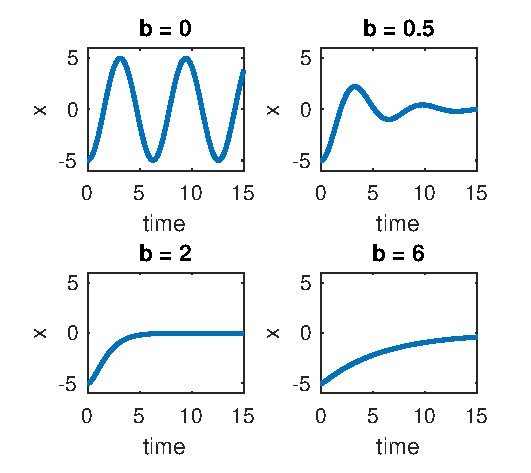
\includegraphics[width=7cm]{figures/ch3/dho_damping.pdf}
\caption{Consequences of scaling the parameter $b$ (damping) in the harmonic oscillator.}
\label{fig:dho_damp}
\end{figure}

\hspace*{-1mm}Finally, $x_0$ denotes equilibrium or resting position. Figure \ref{fig:dho_rest} gives an over\-view of the consequences of manipulating this parameter for a critically damped system. As illustrated by the plots, for a critically damped system or an overdamped system, the parameter $x_0$ is the position of the point attractor that the system converges to. In Articulatory phonology, the control of a tract variable is modelled with a critically damped harmonic oscillator. The resting position $x_0$ corresponds to the constriction location or degree depending on the tract variable. 

\begin{figure}
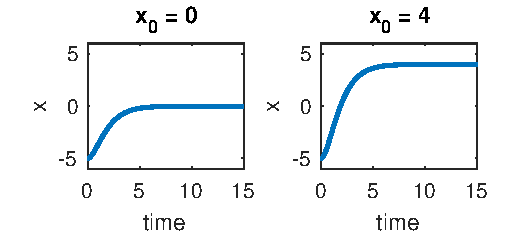
\includegraphics[width=7cm]{figures/ch3/dho_x0.pdf}
\caption{Consequences of scaling the parameter $x_0$ (equilibrium position) in the harmonic oscillator.}
\label{fig:dho_rest}
\end{figure}

In fact, a critically damped harmonic oscillatory never reaches its resting position but only approaches it infinitesimally close. For a concrete implementation scenario of the model, a point has to be defined at which the target is said to be reached. As shown above, an undamped oscillator repeats in even cycles and its oscillation can be described by the phase angle as already shown for the finger movements when discussing the \citet{HakenKelsoBunz1985} model. Articulatory phonology defines the target of the critically damped oscillator as the point of 240° of the undamped corresponding oscillator \citep{BrowmanGoldstein1990}, as shown in Figure \ref{fig:dho_240}. In this figure, one full undamped oscillator cycle is plotted as a solid red line, and the corresponding undamped oscillator is plotted as a dotted blue line. The vertical black line indicates the point where a phase angle of 240° is reached in the cycle of the undamped oscillator, i.e. the \emph{target} of the gesture described by the damped harmonic oscillator. The second x-axis on the bottom relates the time points on the first x-axis to the phase angles in degrees.

\medskip\noindent\textit{Code used in this section: \\
damped\_harmonic\_oscillator.m, damped\_harmonic\_oscillator\_target.m}

\begin{figure}
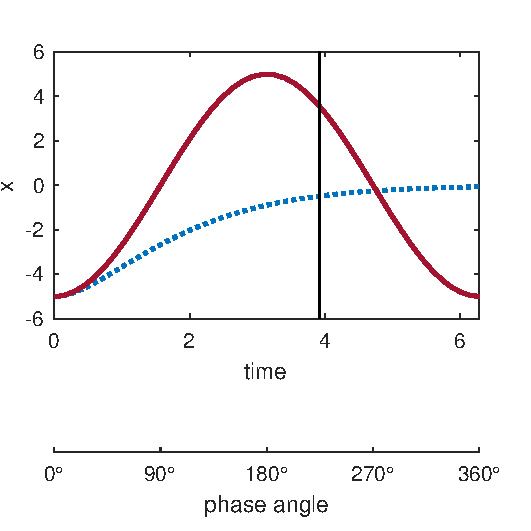
\includegraphics[width=7cm]{figures/ch3/target_240_degrees.pdf}
\caption{The target of the critically damped harmonic oscillator is reached at 240° of the phase angle of the corresponding undamped oscillator.}
\label{fig:dho_240}
\end{figure}

\subsubsection{Inter-gestural timing}

Articulatory phonology views words and syllables as made up of gestures. Although timely ordered in some sense, these gestures are, crucially, not ``beads on string" \citep{Pouplier2011}, i.e. they are not strictly sequentially ordered. Structures like words and syllables should rather be seen as molecular structures \citep{NamGoldsteinSaltzman2009} consisting of gestures and connections between the gestures that determine their relative timing. This section will shed some light on the modelling of timing in Articulatory phonology. Here again, a dynamical systems approach is used which will be reviewed in some detail since it ties together what has been presented in the last two sections on the \citet{HakenKelsoBunz1985} model and the modelling of gestures in Articulatory phonology. 

It has been highlighted in different passages of this work that \emph{timing} is important in the context of  modelling articulatory gestures. The gestural score in Figure \ref{fig:score_late_calls} in Chapter \ref{chapter_pandp} emphasised this fact by showing how fine-grained timing differences can account for more subtle processes, like for example assimilation. To illustrate the point in the present context and for the sake of completeness and clarity, another gestural score is presented in Figure \ref{fig:ban_mad} for the words \emph{ban} and \emph{mad}, adapted from \citet{Goldsteinetal2009}. The only difference between the scores is the timing of the \emph{velar wide} gesture. The result are two completely different words. This simple example demonstrates that the relative timing of the gestures (i.e. the timing of a gesture in relation to another gesture) involved in forming the word plays a significant role in determining phonological structures and lexical contrast. 

\begin{figure}
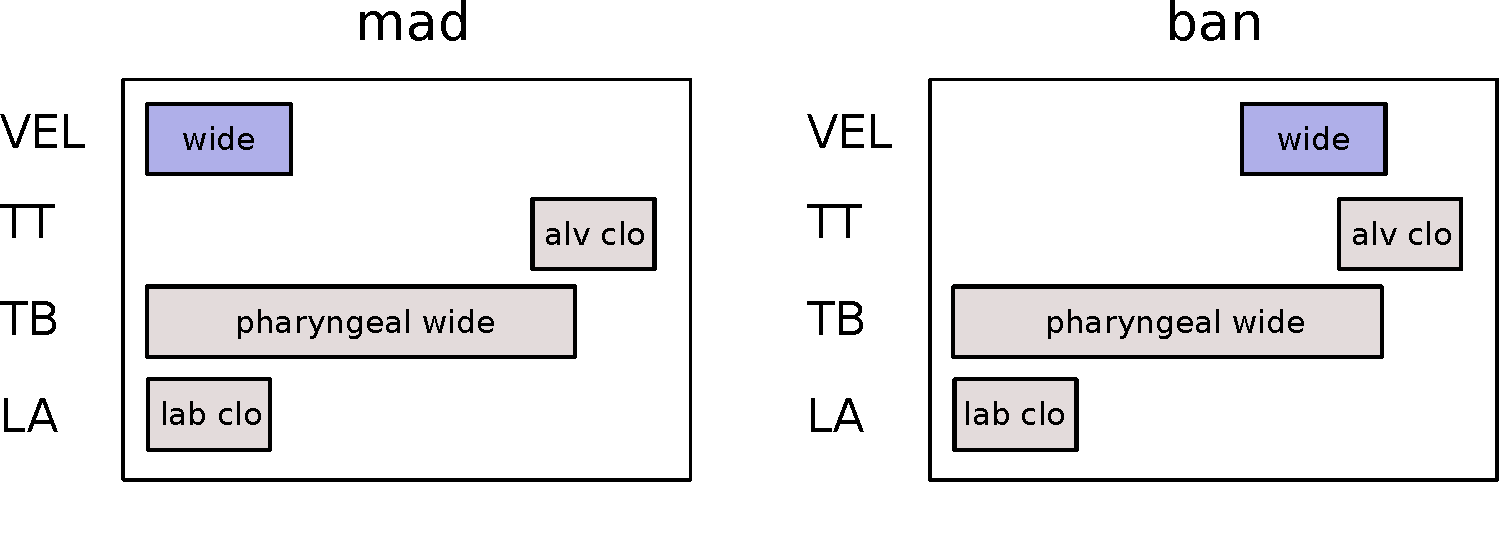
\includegraphics[width=11cm]{figures/ch3/ban_mad.pdf}
\caption{Gestural scores for the words \emph{ban} and \emph{mad} adapted from \citet{Goldsteinetal2009}.}
\label{fig:ban_mad}
\end{figure}

The timing structure of articulatory gestures has been described in detail in a model using \emph{coupled oscillators} \citep{SaltzmanByrd2000, NamSaltzman2003, Goldsteinetal2009, Tilsen2017}. The central idea of this model is that each gesture is associated with a planning oscillator. This planning oscillator is not to be confused with the oscillator that describes the trajectory of the gesture itself. The planning oscillators of multiple gestures are connected with a coupling relation that determines the relative phases of the gestures. As in the model of \citet{HakenKelsoBunz1985}, the two stable patterns of the relative phasing are in-phase and anti-phase. During planning, the oscillators adjust their phases either in an in-phase or anti-phase manner. When a stable pattern is achieved, the actual production gestures are activated by the oscillators. The adjustment of the oscillators towards a stable pattern is modelled using a potential function similar to that of \citet{HakenKelsoBunz1985}. There exist slightly different ways to formulate the coupled oscillator model \citep{SaltzmanByrd2000, Tilsen2017}. \citet{Tilsen2017} presents the potential functions as formulated in \ref{eq:coupled_osc_potential}, where $V^+$ is the potential for  in-phase coupling and $V^-$ is the potential for anti-phase coupling (as in the model of \citeauthor*{HakenKelsoBunz1985}, $\phi$ is relative phase of the oscillators, given as the difference between the individual phases $\theta$: $\phi_{ij} = \theta_i - \theta_j$). The evolution of the relative phase  can be described using the negative derivative of the potential, the force function of the system, as given in Equation \ref{eq:coupled_osc_force}.

\begin{equation}
\begin{split}
V^+(\phi) = -\cos\phi, \quad\quad
V^-(\phi) = \cos\phi
\label{eq:coupled_osc_potential}
\end{split}
\end{equation}

\begin{equation}
F(\phi) = -\frac{dV(\phi)}{d\phi}
\label{eq:coupled_osc_force}
\end{equation}

Each planning oscillator $i$ can be expressed in polar coordinates with the phase $\theta_i$ such that the evolution of planning oscillator's phase without coupling can be described as in Equation \ref{eq:coupled_osc_phase_angle}, where $f_i$ represents the intrinsic frequency of the oscillator \citep{Tilsen2018}.

\begin{equation}
\dot{\theta_i} =  2 \pi f_i
\label{eq:coupled_osc_phase_angle}
\end{equation}

To model the effect of coupling, the expression of Equation \ref{eq:coupled_osc_phase_angle} that models the evolution of the phase angle is extended by the force function of the coupling dynamics $F(\phi)$, see Equation \ref{eq:coupled_osc_phase_angle_with_coupling} \citep{Tilsen2017}. The force that is exerted on the planning oscillator is proportional to the coupling strengths of the planning oscillators. These coupling strengths are given as a matrix in which the coupling strength of each planning oscillator $i$ to another oscillator $j$ is defined. This matrix for three coupled oscillators looks like the one given in Equation \ref{eq:coupled_osc_matrix}. The diagonal elements $c_{ii}$ of the matrix are $0$ because they denote the coupling of the oscillator to itself.

\begin{equation}
\dot{\theta_i} =  2 \pi f_i + \sum_j{ c_{ij} \frac{-dV(\phi_{ij})}{d\phi_{ij}}}
\label{eq:coupled_osc_phase_angle_with_coupling}
\end{equation}

\begin{equation}
C = 
\begin{pmatrix}
0 & c_{12} & c_{13} \\
c_{21} & 0 & c_{23} \\
c_{31} & c_{32} & 0 \\
\end{pmatrix}
\label{eq:coupled_osc_matrix}
\end{equation}

Figure \ref{fig:coupled_oscillators} provides an example of two oscillators that are coupled in an in-phase manner and that start with a relative phase of 110°. The three rows of the figure show three different points in time. The first row presents a time point that is shortly after the beginning of the simulation, the relative phase at this time point is still close to the initial relative phase of 110°. The last row presents a time point at which the two oscillators have almost the same phase, i.e. the relative phase is close to 0°. The middle row presents a time point in between. In the left column, the graph of the potential function is shown with the red dot indicating the current state of the system (it is possible to think of the dot as the ball in the metaphor used above). In the mid column, the phase angles of the oscillators are presented. In the right column, the position of the oscillators are shown in a time window around the time point corresponding to the potential and the phase angles in the same row (the dashed line specifies this time point). The plot illustrates how the state of the system approaches the attractor at 0°, the minimum of the potential, and how the relative phase of the two oscillators decreases over time. 

\begin{figure}
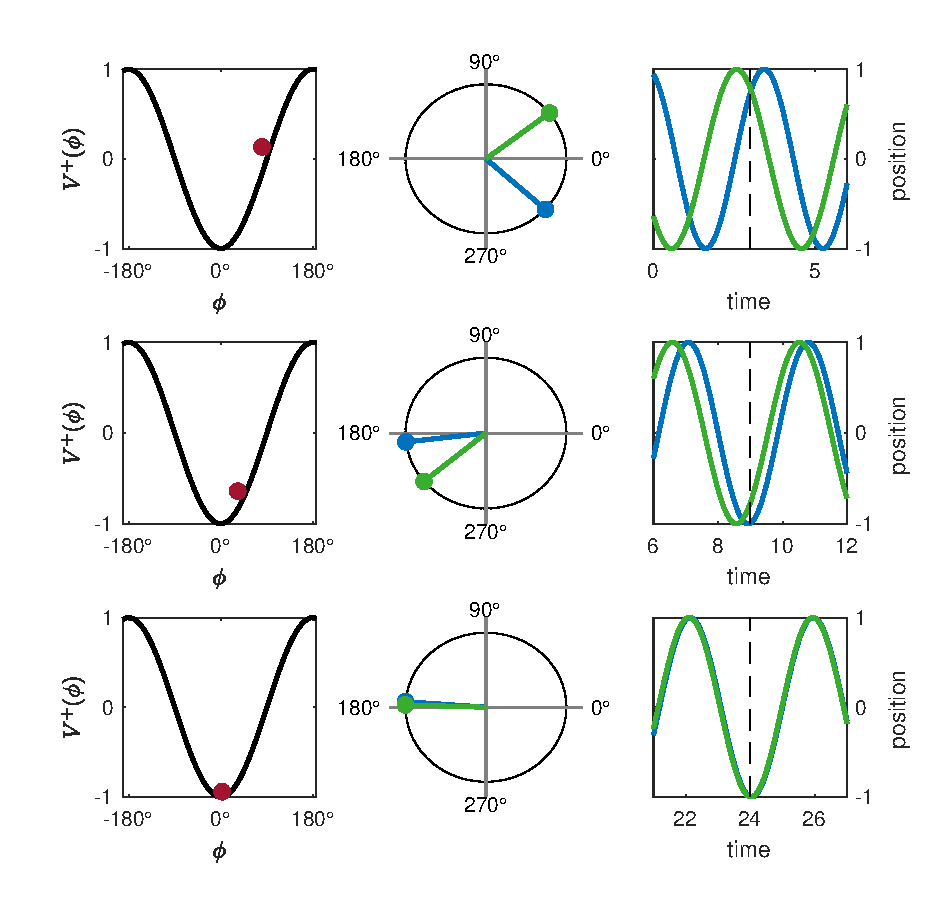
\includegraphics[width=\textwidth]{figures/ch3/coupled_oscillators.pdf}
\caption[Potential, phase angles and position corresponding to two oscillators coupled in-phase]{Potential, phase angles and position corresponding to two oscillators coupled in-phase at three time points (from top to bottom).}
\label{fig:coupled_oscillators}
\end{figure}

Usually, syllables involve more than two gestures and, thus, more than two oscillators are coupled in a pair-wise fashion. As a result, a network of coupled oscillators emerges.\footnote{An alternative view is that the oscillator of each gesture is coupled to a master clock. This perspective is discussed in relation to the network of coupled oscillators in \citet{Goldsteinetal2009}.} The target phasing relations of these oscillators are represented in \emph{coupling graphs}. The coupling graphs for the English words \emph{bud} [bʌd] and \emph{dub} [dʌb], adapted from \citet{Mücke2018}, are shown in Figure \ref{fig:bud_dub}. The solid lines indicate in-phase coupling, the dashed lines indicate anti-phase coupling. The onset consonant of the syllable in both cases is modelled as being coupled in-phase with the vowel of the syllable while the coda consonant is coupled anti-phase with the vowel. This organisation reflects the fundamental hypothesis that CV structures in a syllable are coupled in-phase while VC structures are coupled anti-phase \citep{GoldsteinByrdSaltzman2006, Goldsteinetal2009}.

\begin{figure}
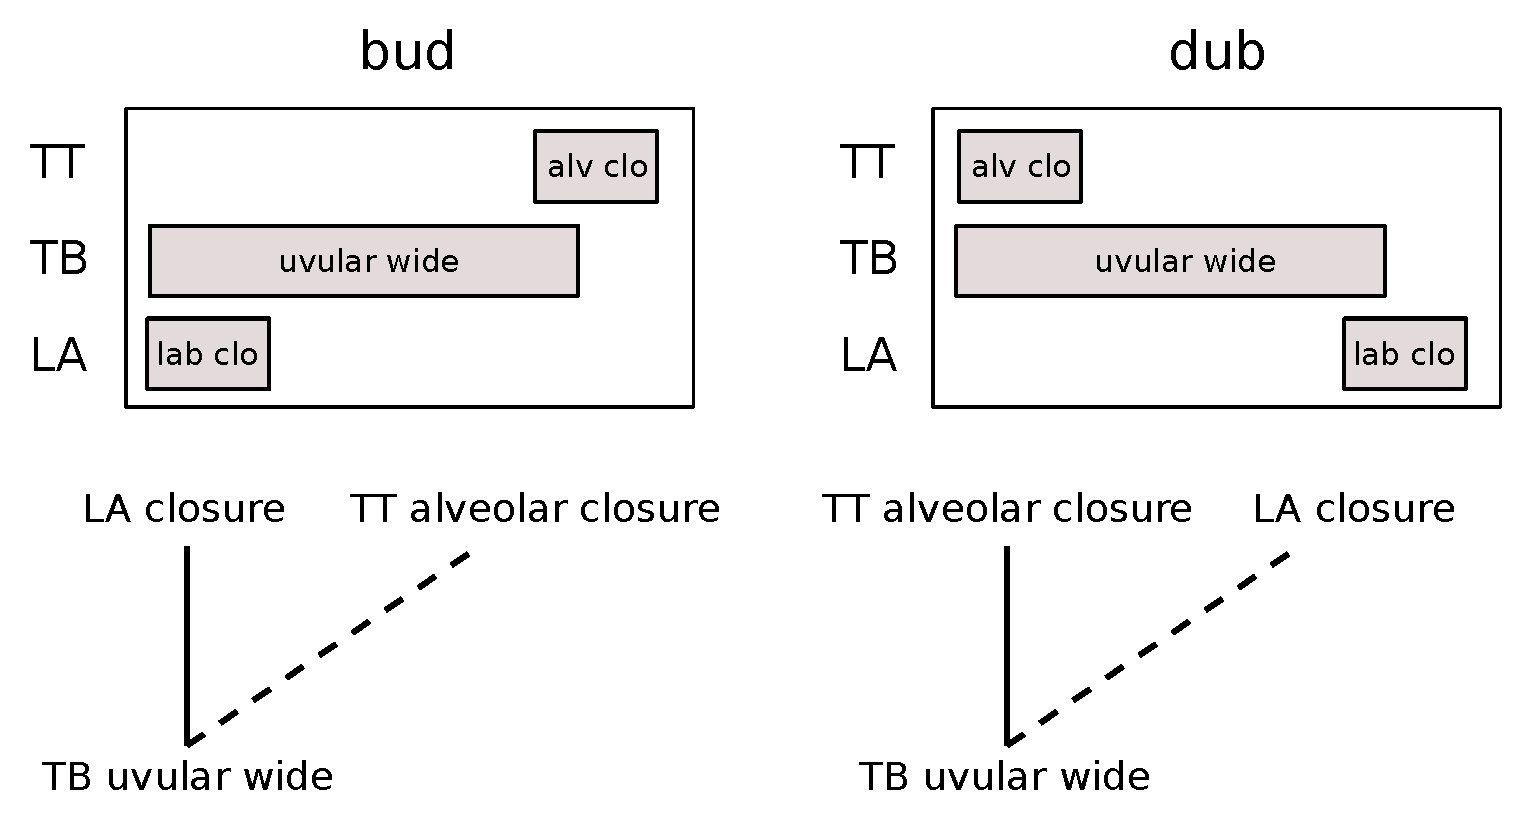
\includegraphics[width=11cm]{figures/ch3/bud_dub.pdf}
\caption[Gestural scores and coupling graphs for \emph{bud} and \emph{dub}.]{Gestural scores and coupling graphs for \emph{bud} [bʌd] and \emph{dub} [dʌb] adapted from \citet{Mücke2018}, solid lines indicate in-phase coupling, dashed lines indicate anti-phase coupling.}
\label{fig:bud_dub}
\end{figure}

If two consonants or more are present in the onset of a syllable, a pair-wise in-phase coupling of all of the consonants to the vowel alone would lead to an overlapping of the consonants. To achieve at least a partially sequential realisation of the onset consonants, the onset gestures of each consonant can be coupled with anti-phase links to the vowel. The result is a \emph{competitive coupling} in which the final phases represent a compromise of the competing coupling forces \citep{Nam2007, Saltzmanetal2008, Goldsteinetal2009}. Competitive coupling is able to explain an effect known as the \emph{C-centre effect} in branching onsets \citep{BrowmanGoldstein1988, Byrd1995}. The C-centre effect, illustrated in Figure \ref{fig:c-centre}, describes the following situation: The timing of C1 in relation of the vowel V in a complex onset structure C1C2V is earlier compared to the simple structure C1V. In other words, when a second consonant C2 is added after C1, the earlier consonant C1 shifts leftwards. Likewise, the timing of C2 in C1C2V is later compared to the simpler structure C2V, i.e. when a second consonant C1 is added before C2, the later consonant C2 shifts rightwards. The timing of the centre of the consonant cluster in relation to the vowel, however, stays constant \citep{BrowmanGoldstein1988, Goldsteinetal2009}.

\begin{figure}
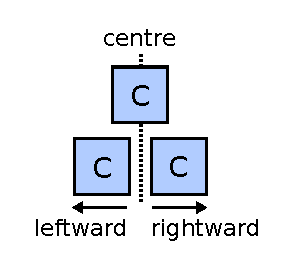
\includegraphics[width=3.5cm]{figures/ch3/c_centre.pdf}
\caption{Schematic illustration of the c-centre effect adapted from \citet{HermesMückeGrice2013}.}
\label{fig:c-centre}
\end{figure}

\medskip\noindent \textit{Code used in this section: coupled\_osc.m}

\subsection{Modelling dynamics of categoriality and continuity}

In the last section, dynamical models of motion and articulation have been presented. Crucially, these models do not only entail mere physical descriptions of the mechanism of speech production but put the dynamical approach they employ in a phonological, cognitive perspective: The gestures of Articulatory phonology are viewed as phonological primitives, the coordination patterns of the coupled oscillators model shape phonological patterns of syllable structure. This perspective maintains that both categorical aspects and continuous aspects of speech can be described jointly by dynamical models. The current section explores this idea more explicitly by presenting some interesting and influential approaches to modelling categoriality and continuity in the sound pattern of language.

\subsubsection{Perceptual categories}

\citet{Tulleretal1994} present a dynamical model that is able to account for interesting results in the perception of speech sound categories. Their work illustrates how the stability of speech sound categories and their perception can be modelled while including flexibility of the perceptual responses.

The authors exposed participants to ordered continua between English \emph{say} and \emph{stay} and between \emph{stay} and \emph{say}. To be more specific, the gap duration between \emph{s} and \emph{ay} increases and then decreases with each stimulus during one experiment run. The participants were tasked to categorise each stimulus in a forced choice task. Two dominant response patterns are evident in the data. In one response pattern, the category switch in the increasing order (the gap duration becomes larger) is later compared to the decreasing order (the gap duration becomes smaller). In other words, for the change from \emph{say} to \emph{stay} a larger gap is necessary than for the change from \emph{stay} to \emph{say}. This response pattern is called \emph{hysteresis}. In the other response pattern, the category switch is earlier in the increasing order compared to the decreasing order. For the change from \emph{say} to \emph{stay} a smaller gap is necessary than for the change from \emph{stay} to \emph{say}. This response pattern is called \emph{enhanced contrast}. Both patterns are illustrated in the two top panels of Figure \ref{fig:tuller_response}. The figure also shows the response pattern \emph{critical boundary} in which the category switch occurs at the same point in the acoustic continuum in both increasing and decreasing order. In the data of \citet{Tulleretal1994}, the response patterns hysteresis and enhanced contrast dominate while the pattern critical boundary is rarely found.

\begin{figure}
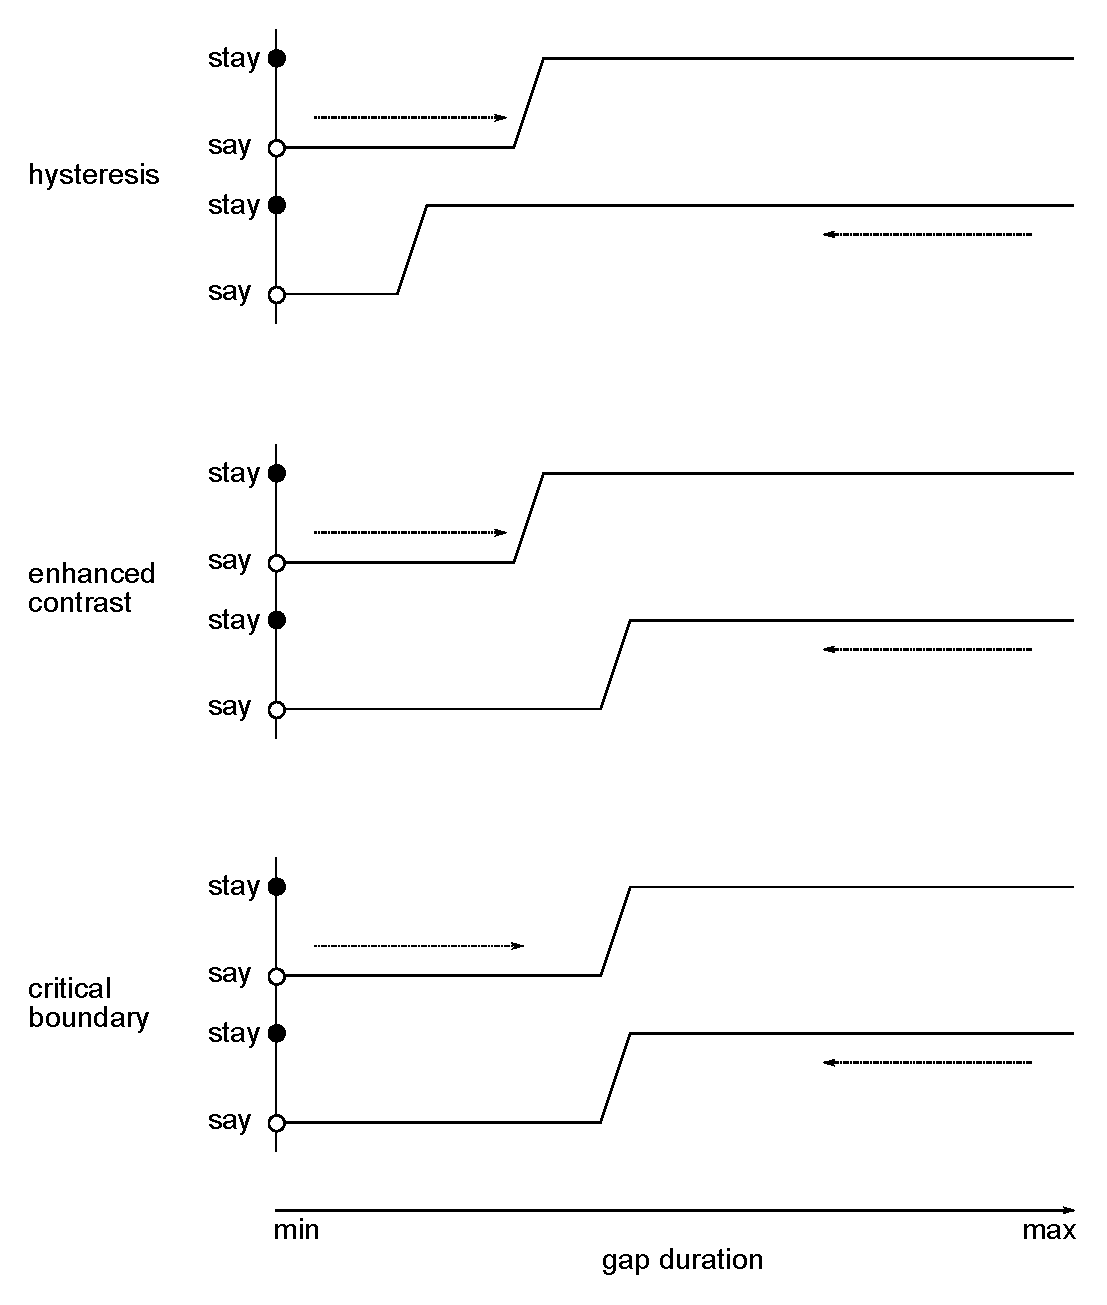
\includegraphics[width=11cm]{figures/ch3/tuller_etal_1994_response_patterns.pdf}
\caption[Possible response patterns of \citet{Tulleretal1994}.]{Possible response pattern of \citet{Tulleretal1994}: hysteresis (top), enhanced contrast (middle), critical boundary (bottom).}
\label{fig:tuller_response}
\end{figure}

\citet{Tulleretal1994} propose a model that is similar to the double well potential introduced in the first part of the chapter in Equation \ref{eq:double_well_potential} and illustrated in Figure \ref{fig:double_well_potential} with a slight difference: The control parameter $k$ occurs with a positive sign in the present model, see Equation \ref{eq:tuller_potential_equation}. The effect of this difference is simply that the scaling of the control parameter has the opposite effect. For positive $k$ values, e.g. $k = 1$, the landscape is tilted to the left, for negative $k$ values, e.g. $k = -1$, it is tilted to the right. 
To connect this attractor landscape to the perceptual data, one attractor is associated with the percept of \emph{say}, the other with \emph{stay}, see Figure \ref{fig:tuller_potential}. While listening to the ordered continuum from \emph{say} to \emph{stay}, the control parameter increases and the attractor landscape gradually tilts to the side of \emph{stay}. When the critical boundary $k_c$ is reached, the \emph{say} attractor is destabilised and the percept changes to \emph{stay}. The process takes place analogously from \emph{stay} to \emph{say} when the control parameter decreases (in this case, the critical boundary is $-k_c$).

\begin{equation}
V(x) = kx - \frac{x^2}{2} + \frac{x^4}{4}
\label{eq:tuller_potential_equation}
\end{equation}

\begin{figure}
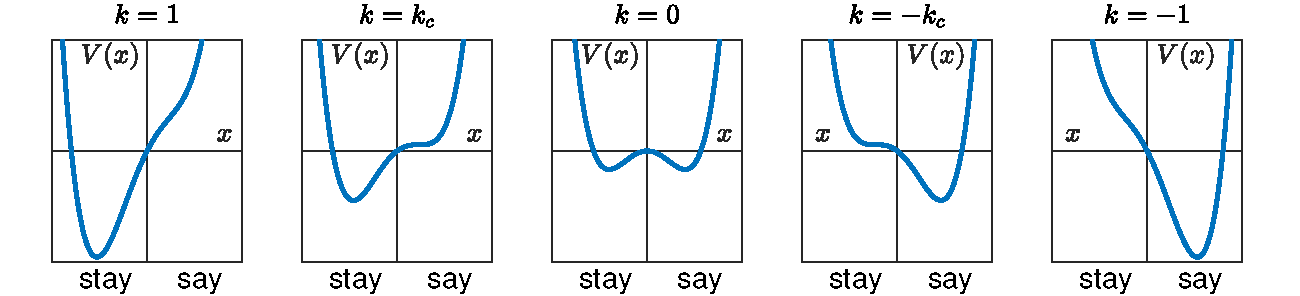
\includegraphics[width=\textwidth]{figures/ch3/tuller_potential.pdf}
\caption{Potential function of \citet{Tulleretal1994} for different values of the control parameter $k$.}
\label{fig:tuller_potential}
\end{figure}

In the response patterns described above, the switch from one category to the other (i.e. \emph{say} to \emph{stay} or \emph{stay} to \emph{say}) is at different points in the continuum. For the model, this means that the critical value of the control parameter $k$ in both sides (towards \emph{stay} or towards \emph{say}) has to occur with different gap durations in the response patterns. To explain this phenomenon, \citet{Tulleretal1994} hypothesise that $k$ depends on a variety of variables and is determined by the function given in Equation \ref{eq:tuller_k_formula}. In this function, $k_0$ is the value of $k$ at the beginning of the run, i.e. $-1$ when the participant starts listening to the continuum with increasing gap durations from \emph{say} to \emph{stay}. $\lambda$ is a variable that is proportional to the gap duration and thus represents the position on the acoustic continuum. $\lambda_f$ is the value of $\lambda$ at the other end of the continuum, i.e. the maximal gap duration when the trial starts with \emph{say} (without a gap). The variable $n$ represents the number of stimuli that the participant already listened to, $n_c$ denotes a critical number of trials defined as 50\% of the trials. $\theta(n-n_c)$ is a step function that is defined as $0$ when $n < n_c$, i.e. in the first half of the trial, and $1$ when $n \geq n_c$, i.e. in the second half of the trial. The variable $\epsilon$ ``represents the lumped effect of learning, linguistic experience, and attentional factors” \citep[8]{Tulleretal1994}. This last parameter is a very important parameter for the model because it plays a major role in explaining the response patterns introduced above.

\begin{equation}
k(\lambda) = k_0 + \lambda + \frac{\epsilon}{2} + \epsilon\theta(n-n_c)(\lambda-\lambda_f)
\label{eq:tuller_k_formula}
\end{equation}

Figure \ref{fig:tuller_colour_map} provides an illustration of the relation between $\epsilon$, gap duration represented by $\lambda$ and the control parameter $k$ as a colour map. The colours represent the values of $k$ determined with the formula of Equation \ref{eq:tuller_k_formula}. The left plot presents the predictions for the first half of the run (increasing gap durations), the right plot presents the predictions for the second half of the run (decreasing gap durations). The colours are only shown for the range of $k$ values in the interval of $[-1, 1]$. Of course $k$ further increases (left plot) or decreases (right plot) through the white area but the restriction to this range makes the colour contrasts stronger and thus visualises the differences better. Both plots show that the colours reflecting the values of the control parameter $k$ are distributed roughly diagonally over the plots. This structure illustrates that for the same gap durations, $k$ values are higher when $\epsilon$ is large in the first half of the run. The opposite is true for the second half of the run where $k$ values are lower when $\epsilon$ is large. 

\begin{figure}
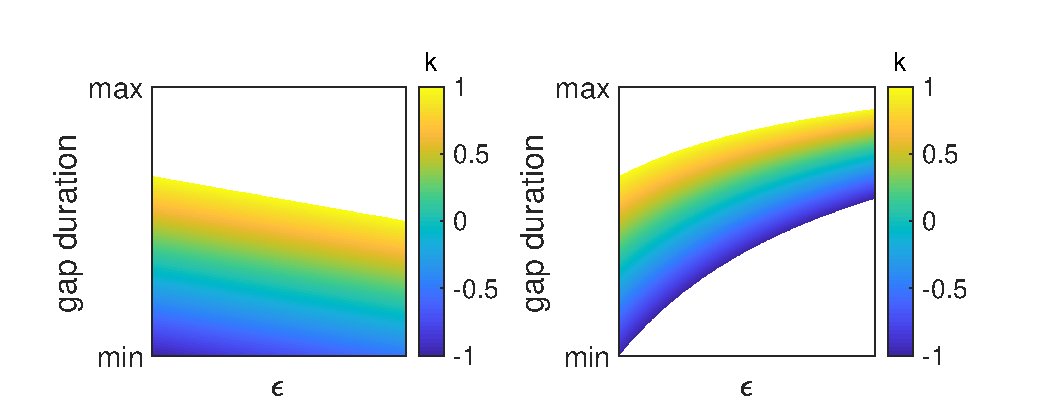
\includegraphics[width=12cm]{figures/ch3/tuller_map.pdf}
\caption[Colour maps representing the values for the control parameter $k$ in relation to $\epsilon$ and gap duration in the \citet{Tulleretal1994} model.]{Colour maps representing the values for the control parameter $k$ in relation to $\epsilon$ and gap duration in the \citet{Tulleretal1994} model. Left: first half of the run with increasing gap durations (small $n$). Right: second half of the run with decreasing gap durations (large $n$).}
\label{fig:tuller_colour_map}
\end{figure}

Recall that the system stays in the attractor as long as the critical value of $k$ that destabilises the attractor is not crossed. When it is crossed, the system moves to the remaining attractor and the percept changes. In a forced choice experiment, the participant changes the response at that point. It is thus sensible to investigate which value of $\lambda$, i.e. which gap durations, yield the critical value of $k$ for different values of $\epsilon$. The thick lines in Figure \ref{fig:tuller_lambda_epsilon} show at which gap duration (y-axis) the critical boundary $k$ occurs as a function of $\epsilon$ (x-axis). The shaded area in the left and middle panel is the span of gap durations for which the system has two attractors, i.e. the control parameter $k$ is between the critical values on both sides $-k_c$ and $k_c$.

The left panel of \ref{fig:tuller_lambda_epsilon} presents the predictions for the first half of the run. The plot is to be read from bottom to top as the arrows indicate, i.e. from no gap to the maximal gap duration (\emph{say} to \emph{stay}). The number of perceived stimuli $n$ is small in this first half and under the threshold  $n_c$ (and thus $\theta(n-n_c) = 0$). When $\epsilon$ is small (left on the x-axis), the categorisation is only dependent on the gap duration. However, for larger $\epsilon$ values, the gap duration needed to shift the percept from \emph{say} to \emph{stay} decreases. In other words, the larger $\epsilon$, the earlier the switch from one category to the other when going from no gap to the maximum gap.

The middle panel of \ref{fig:tuller_lambda_epsilon} shows the predictions for the second half of the run. This plot is to be read from top to bottom, i.e. from the maximal gap duration to no gap (\emph{stay} to \emph{say}). The number of perceived stimuli in the second half is large and above the threshold $n_c$ (and thus $\theta(n-n_c) = 1$). In this case, the model predicts that for larger $\epsilon$ values, the gap duration needed to switch the percept from \emph{stay} to \emph{say} is larger compared to smaller values of $\epsilon$. The larger $\epsilon$, the earlier the switch from from \emph{stay} to \emph{say} when going from the maximum gap to no gap.

The right panel of \ref{fig:tuller_lambda_epsilon} combines the thick lines of the two neighbouring plots. There is a critical value of $\epsilon$, namely $\epsilon_c$, for which the category switch occurs at the same gap duration in both halves of the run. At this point the two lines intersect. When $\epsilon$ is below $\epsilon_c$, the percept changes later and the observed response pattern is \emph{hysteresis}. This is visualised by the line of the first half of the run being positioned above the line of the second half of the run. Going from bottom (no gap) to top (maximum gap) in the first half of the run, the critical boundary of $k$ is reached at a longer gap duration. Going from top (maximum gap) to bottom (no gap) in the second half of the run, the critical boundary of $k$ is reached at a shorter gap duration. 

When $\epsilon$ is above the critical $\epsilon_c$, the percept changes earlier and the observed response pattern is \emph{enhanced contrast}. This is illustrated by the fact that the line of the first half of the run  is positioned under the line of the second half of the run. Going from bottom (no gap) to top (maximum gap) in the first half of the run, the critical boundary of $k$ is reached at a shorter gap duration. Going from top (maximum gap) to bottom (no gap) in the second half of the run, the critical boundary of $k$ is reached at a longer gap duration.

\begin{figure}
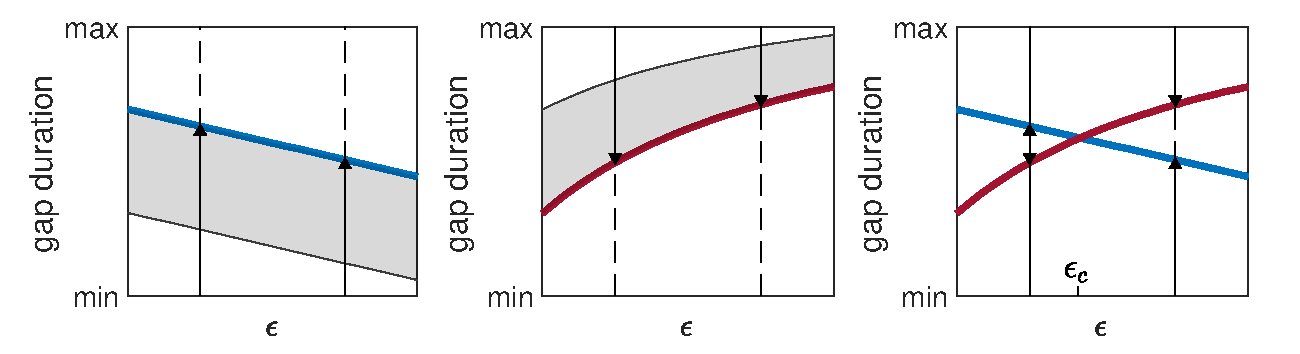
\includegraphics[width=\textwidth]{figures/ch3/tuller_lambda_epsilon_plane.pdf}
\caption[Location of critical values of the control parameter $k$ in the acoustic continuum of gap duration as a function of the parameter $\epsilon$ in the \citet{Tulleretal1994} model.]{Location of critical values of the control parameter $k$ in the acoustic continuum of gap duration as a function of the parameter $\epsilon$ in the \citet{Tulleretal1994} model. Left: first half of the run (increasing gap duration, small $n$). Middle: second half of the run (decreasing gap duration, large $n$). Right: superposition of critical boundary in first and second run.}
\label{fig:tuller_lambda_epsilon}
\end{figure}

The model of \citet{Tulleretal1994} shows how the flexibility and context dependency of perceptual categories can be modelled using the double well potential with two attractors presented earlier in this chapter. The next section will present work adapting a similar potential for the modelling approach to capture continuous and categorical variation found in production data.

\medskip\noindent \textit{Code used in this section:\\
tuller\_1994\_potential.m, tuller\_1994\_crit\_lambda.m, tuller\_1994\_map.m}

\subsubsection{Incomplete neutralisation}

As introduced in the previous chapter, the phenomenon of incomplete neutralisation of syllable final obstruents in German poses a major problems for purely symbolic approaches to phonology and a modular separation of phonetics from phonology. To remind the reader, a large body of work has centred around the question whether the voicing contrast of obstruents in syllable coda positions in German is complete or not. Numerous studies have shown that there are indeed differences between the final obstruents of words like \emph{Rat} and \emph{Rad} such that the acoustic features of the devoiced final obstruent [t] in \emph{Rad} are modulated subtly in the direction of the voiced [d].

In addition, a study by \citet{PortCrawford1989} suggests that the communicative context modulates the differences between the obstruents. When the speaker produces the words containing the obstruents in direct contrast (``Ich habe Rad gesagt, nicht Rat") and a listener is tasked to write down the correct word, the supposedly neutralised obstruent shifts more in the direction of the voiced variant compared to a task in which the speaker simply reads the words in a list.

\citet{GafosBenus2006} propose a dynamical model that is able to capture the differences between the obstruents in relation of the speaker's intent to maintain the contrast. In this model, the categorical nature of the phonological voicing contrast can be maintained while allowing for fine-grained differences. In the first part of the model, the intention of a speaker to produce a voiced or a voiceless obstruent is described by defining one attractor for each voicing value on a continuum of voicing. The continuum of voicing are all possible states $x$ of the systems. The intention to produce a contrast is formally modelled with the force function $F(x)$ in Equation \ref{eq:gafos_benus_intentional_force_potential}, where $x_{req}$ is the \emph{required} (i.e. intended) value on the voicing continuum $x$. Crucially, $x_{req}$ is the location of the attractor of this system. For the voiceless obstruent, a location in the positive range of $x$ denoted by $x_0$ is chosen. For the voiced obstruent, a location the negative range of $x$ denoted by $-x_0$ is chosen. The exact values do not play a role in the modelling approach, it is only important that they are distributed on both sides of zero.

The second line of Equation \ref{eq:gafos_benus_intentional_force_potential} presents the potential energy function $V_F(x)$ that is obtained by integration of the negative of the force function. Figure \ref{fig:gafos_benus_intentional_force_potential} displays $F(x)$ and $V_F(x)$ with $x_{req} = -x_0$ on the left and $x_{req} = x_0$ on the right. The control parameter of this system is $\theta$, a quantity representing the intent of the speaker to produce this value of voicing $x_{req}$. In the further description of the model, the role of the parameter $\theta$ will become clearer.

\begin{equation}
\begin{split}
F(x) = \theta (x_{req} - x) \\
V_F(x) = \theta \frac{x^2}{2} -\theta x_{req} x
\end{split}
\label{eq:gafos_benus_intentional_force_potential}
\end{equation}

\begin{figure}
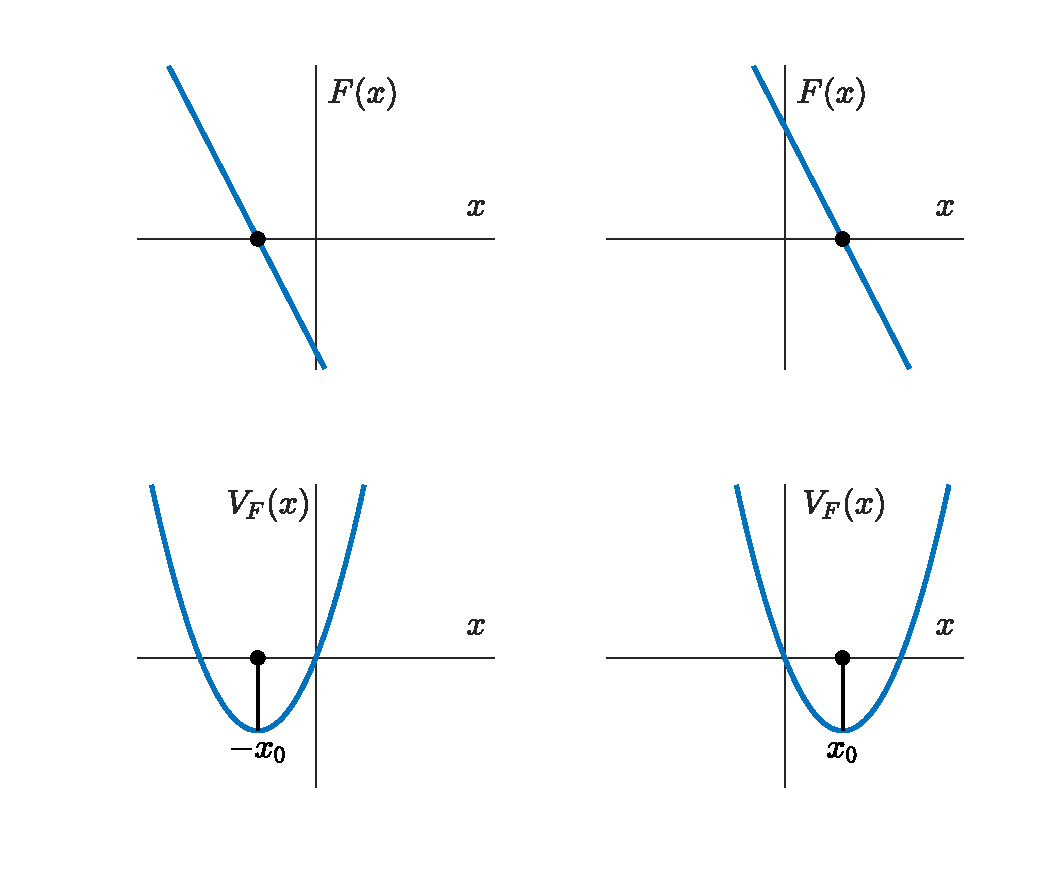
\includegraphics[width=10cm]{figures/ch3/gafos_benus_intentional_dynamics.pdf}
\caption[Force and potential for voiced and voiceless obstruents in the \citet{GafosBenus2006} model.]{Force (top) and potentials (bottom) for $x_{req} = -x_0$ (voiced) and $x_{req} = x_0$ (voiceless) in the \citet{GafosBenus2006} model. Vertical lines in the potential visualise the location of the minimum at the value of $x_{req}$ ($-x_0$ or $x_0$).}
\label{fig:gafos_benus_intentional_force_potential}
\end{figure}

In the second part of the model, an additional force is introduced to account for the fact that German allows for voiceless obstruents only in syllable coda. Here, the same attractor landscape is used as in \citet{Tulleretal1994}, its force $M(x)$ and potential $V_M(x)$ are given in Equation \ref{eq:gafos_benus_coda_force_potential}. For the control parameter $k$, a value beyond the critical threshold of $-k_c$ is chosen ($-1$ in the illustration) such that the landscape is tilted to the voiceless side and the voiceless attractor is the only attractor that remains, see Figure \ref{fig:gafos_benus_coda_potential}. The presence of only on attractor reflects the fact that there is one possibility for obstruents in syllable codas: voiceless.

\begin{equation}
\begin{split}
M(x) = -k+x-x^3\\
V_M(x) = kx - \frac{x^2}{2} + \frac{x^4}{4}
\end{split}
\label{eq:gafos_benus_coda_force_potential}
\end{equation}

\begin{figure}
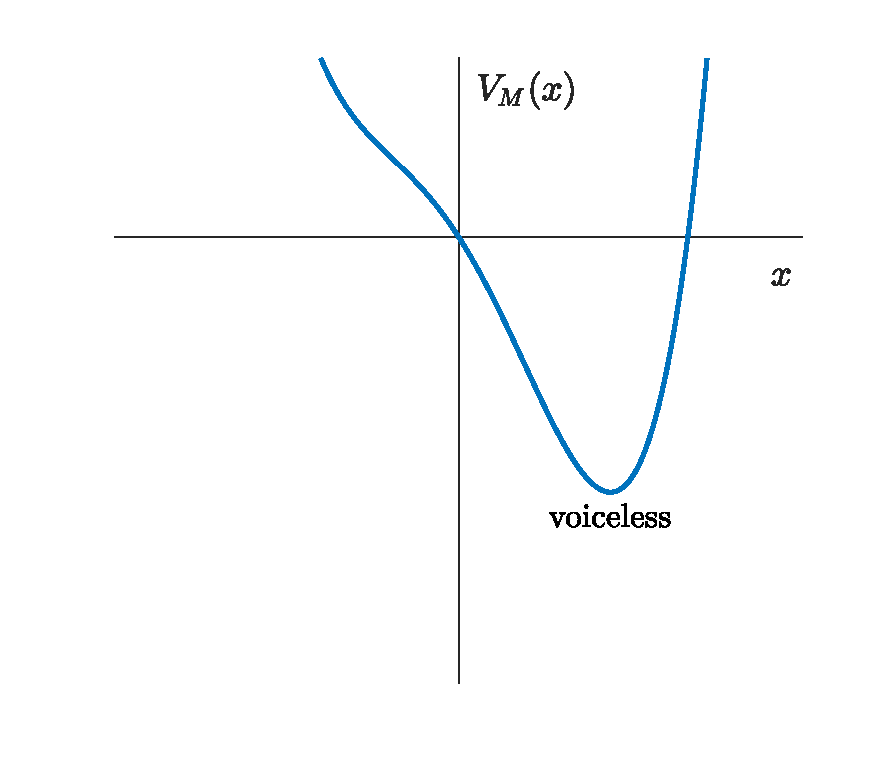
\includegraphics[width=8cm]{figures/ch3/gafos_benus_coda_potential.pdf}
\caption[Tilted double well potential $V_M(x)$ of the \citet{GafosBenus2006} model.]{Double well potential $V_M(x)$ of the \citet{GafosBenus2006} model tilted to the right side to represent the fact that only the voiceless attractor is available in coda position.}
\label{fig:gafos_benus_coda_potential}
\end{figure}

\citet{GafosBenus2006} draw parallels of their dynamical model to an analysis of the phenomenon in optimality theory (OT), a purely symbolic framework. In such an analysis, the presence of one attractor for voiced and one attractor for voiceless obstruents as in the first part of the model corresponds to a \emph{faithfulness} constraint. This constraint is violated when the output form deviates from the underlying representation, see Chapter \ref{chapter_pandp}. In other words, the constraint entails that it is the intention of the speaker to produce outputs as close as possible to the underlying representation. The second part of the model in which only an attractor for voiceless is present corresponds to a \emph{markedness} constraint that requires coda consonants to be voiceless in German.

The interaction of the two parts of the model is achieved by adding up the two forces $F(x)$ and $M(x)$ to obtain the final force function of the system (see Equation \ref{eq:gafos_benus_interaction} for the combined force and potential). In an OT analysis, the markedness constraint would be ranked higher than the faithfulness constraint eliminating any influence of the latter. In the interaction of the present model, however, the force $F(x)$ can influence the outcome of the whole system even if the force $M(x)$ might be stronger. This means that despite the pressure to realise only voiceless obstruents in syllable-final position, the ``underlying" voicing can still have an impact. The size of this impact can be scaled by virtue of a scalar value.

\begin{equation}
\begin{split}
M(x) + F(x) = -k+x-x^3 + \theta (x_{req} - x) \\
V_M(x) + V_F(x) = V(x) = kx - \frac{x^2}{2} + \frac{x^4}{4} + \theta \frac{x^2}{2} - \theta x_{req} x
\end{split}
\label{eq:gafos_benus_interaction}
\end{equation}

The resulting patterns are illustrated in Figure \ref{fig:gafos_benus_combined_potentials}. The top panel presents the outcomes for the underlying voiced obstruent, i.e. $x_{req} = -x_0$, for three possible values of $\theta$: 0.1, 0.3, and 0.5. With increasing $\theta$ the attractor basin drifts subtly towards the negative, voiced part of the continuum $x$ while it stays in the general region of the positive, voiceless part of $x$. As a result, the voiceless obstruent becomes \emph{slighty more voiced}. The production of words like \emph{Rat} with underlyingly voiceless obstruent, i.e. $x_{req} = x_0$, does not lead to the same conflict. The lower panel of Figure \ref{fig:gafos_benus_combined_potentials} shows for the same three values of $\theta$ that the location of the attractor does not change. 

To summarise, producing the intended obstruent and adhering to voiceless obstruents in codas leads to a conflict in words like \emph{Rad}. While this conflict is resolved by a constrain ranking and a single resulting outcome in OT, the interaction can be modulated continuously in the model of \citet{GafosBenus2006}. The effect of $F(x)$ on $M(x)$ is a ``pull" towards more voiced productions on the voicing continuum $x$. This ``pull" is modulated by the scaling of the control parameter $\theta$. 

\begin{figure}
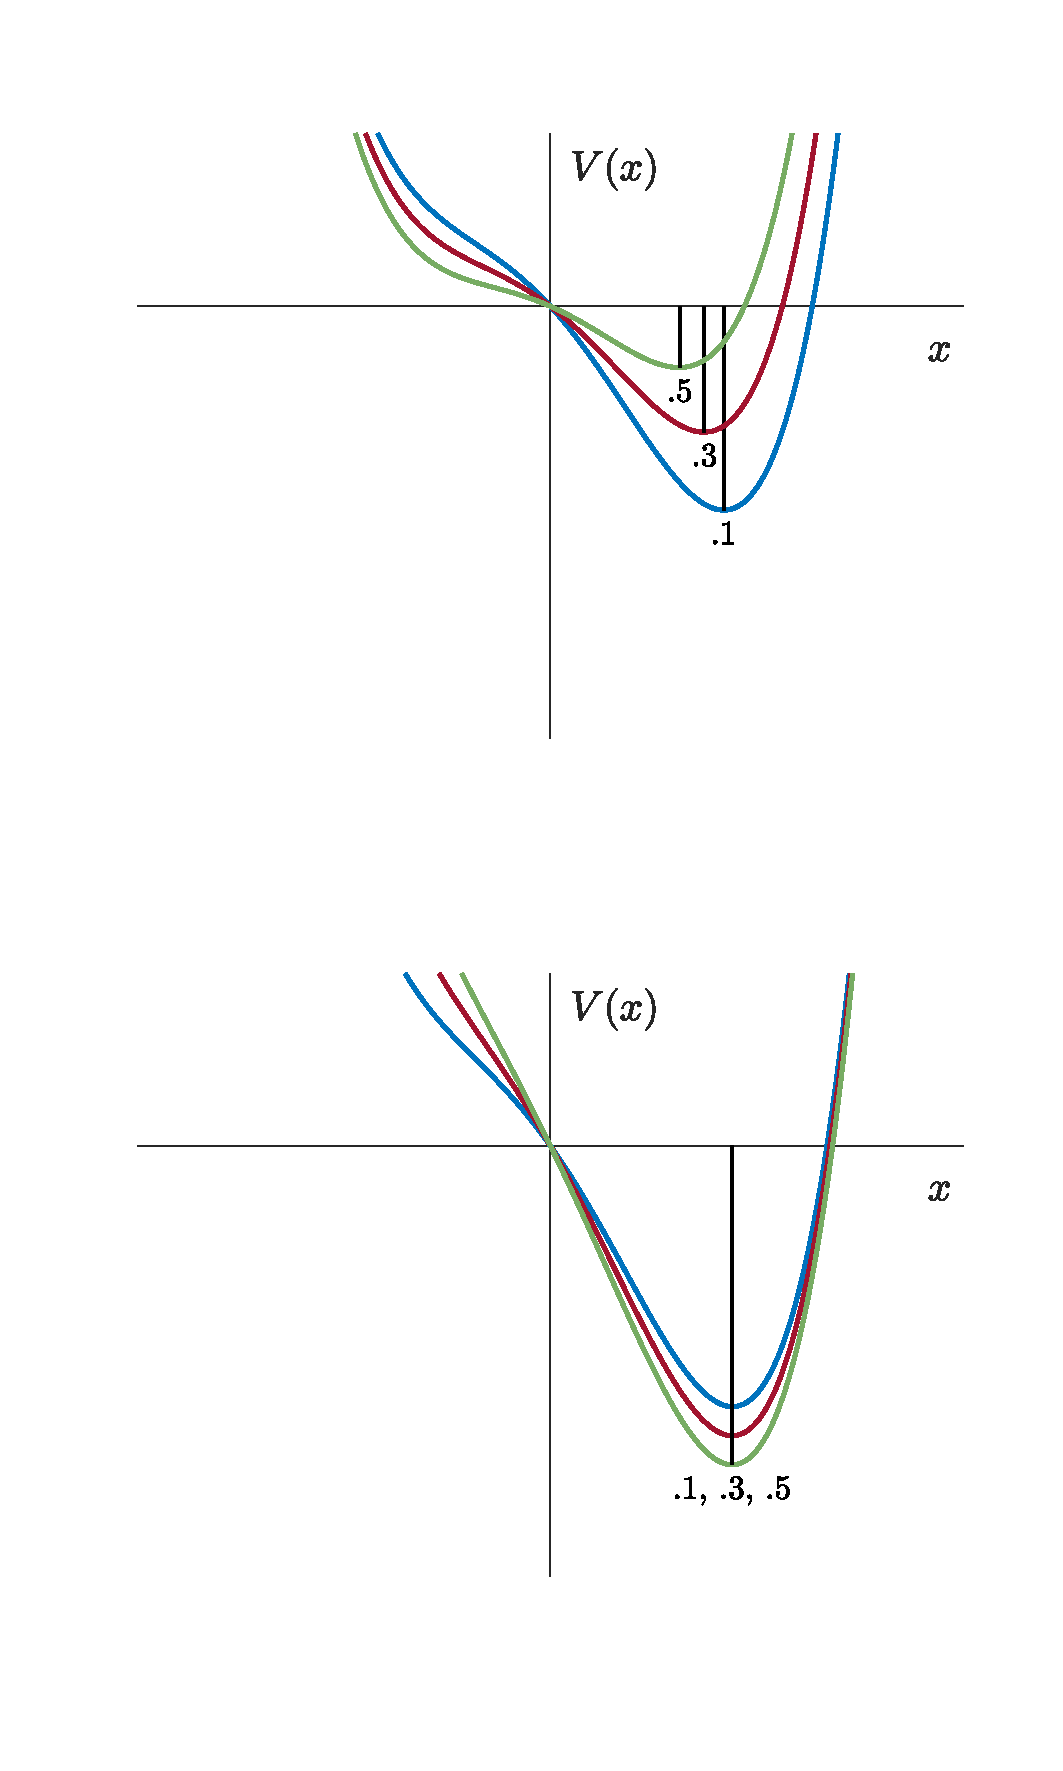
\includegraphics[width=8.5cm]{figures/ch3/gafos_combined_potentials.pdf}
\caption[Combined potentials of the model of \citet{GafosBenus2006}.]{Combined potentials of the model of \citet{GafosBenus2006} for three values of the control parameter $\theta$. Vertical lines indicate the location of the attractor. Blue: $\theta = 0.1$, red: $\theta = 0.3$, green: $\theta = 0.5$. $k$ is constant at $-1$ in all graphs.}
\label{fig:gafos_benus_combined_potentials}
\end{figure}

\medskip\noindent \textit{Code used in this section: gafos\_benus\_incomplete\_neutralisation.m}

\subsubsection{Transparent vowels}

In the previous chapter, the phenomenon of transparent vowels in Hungarian has been introduced. It was explained there that the front unrounded vowels function as transparent vowels as they can occur between the vowel triggering the vowel harmony and the target of the vowel harmony but have been described as not affecting the process of vowel harmony. For example, the back vowel /aː/ of the stem \emph{kávé} /kaːveː/ (`coffee') determines the vowel /ɔ/ of the suffix \emph{nak} /nɔk/ regardless of the intervening unrounded front vowel in the stem. 

The supposedly insignificant role of the transparent vowels in the determination of suffixes, however, is questioned by observations of the behaviour of transparent vowels. Stems that only have transparent vowels can trigger both front and back suffixes \citep{Vago1980, GafosBenus2006} although the distribution of the suffixes is not even, as the majority of stems triggers front suffixes \citep{HayesLonde2006, GafosBenus2006}. In addition, the probability of selecting a back suffix decreases with increasing numbers of transparent vowels intervening between a back stem vowel and the suffix \citep{GafosBenus2006}.

\citet{GafosBenus2006} (as well as \citealp{Benus2005}) hypothesise that systematic articulatory differences in transparent vowels are responsible for the suffix choice. In consequence, transparent vowels may participate in the process of vowel harmony. The authors report data from a study employing electromagnetic articulography and ultrasound to track the position of the tongue and investigate the tongue shape. They show that the tongue is more advanced when articulating transparent vowels in stems that trigger front suffixes compared to transparent vowels in stems that trigger back suffixes. A dynamical model is proposed that resembles the model for incomplete neutralisation outlined in the previous section although the two deal with rather different phonological phenomena. Nevertheless -- like the model for incomplete neutralisation -- the present model links \emph{continuous} and \emph{categorical} aspects in one formal approach.

The first part of the model is a formalisation of articulatory gestures by point-attractor dynamics which is in line with the description of gestures in Articulatory phonology (see also the damped harmonic oscillator presented above). The dynamics of the spatial dimension of constriction location of the tongue body is modelled with a monostable potential as given in its general form in the first line of Equation \ref{eq:gafos_benus_constriction_location}. $x_0$ represents the target constriction location. The factor $\gamma$ represents the strength with which this gesture controls the articulator, the consequence of its scaling will become clearer in the further description. The equation also presents two potentials in the second and third line, one for back vowels and one for front vowels. The factor $\gamma$ is now called $\alpha$ for back vowels and $\beta$ for front vowels. For the back vowel, $x_0$ is chosen as $-2$; for the front vowel, $x_0$ is chosen as $2$. The two potentials $V_B(x)$ (back vowels) and $V_F(x)$ (front vowels) are shown in Figure \ref{fig:gafos_benus_constriction_location_potentials} (with $\alpha = \beta = 1$). 

\begin{equation}
\begin{split}
V(x) = \gamma (x-x_0)^2 \\
V_B(x) = \alpha (x+2)^2 \\
V_F(x) = \beta (x-2)^2
\end{split}
\label{eq:gafos_benus_constriction_location}
\end{equation}

\begin{figure}
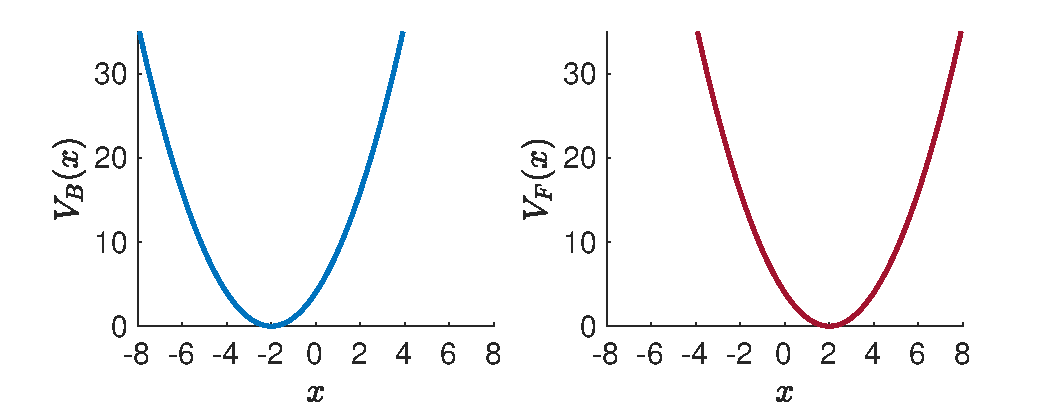
\includegraphics[width=11cm]{figures/ch3/gafos_benus_constriction_location_potential.pdf}
\caption[Monostable potentials modelling the tongue body gesture with regard to constriction location.]{Monostable potentials modelling the tongue body gesture with regard to constriction location. Left: $V_B(x)$ for back vowels, right: $V_F(x)$ for front vowels.}
\label{fig:gafos_benus_constriction_location_potentials}
\end{figure}

The effect of coarticulation of vowels can be modelled as gestural blending by assuming linear combinations of the respective vowel potentials, $V_B(x) + V_F(x)$, and adjusting the values for the factors $\alpha$ and $\beta$. Simply speaking: The factors $\alpha$ and $\beta$ represent weights that specify which gesture will have a dominant effect in the blending. In this way, the influence of a preceding vowel on the target constriction location of a vowel can be captured. Figure \ref{fig:gafos_benus_blending_examples} illustrates two examples for combined potentials produced by linear combinations of the vowel potentials for different values of $\alpha$ and $\beta$. In this figure, the solid lines represent the two potentials for back and front vowels $V_B(x)$ and $V_F(x)$ as in the previous figure. The dotted line shows the graph of the combined potential: $V_B(x) + V_F(x)$. The position of the minimum of this graph on the $x$ axis indicates the vowel target that results from the blending. In the left panel, the case $\alpha = \beta = 1$ is shown, the hypothetical vowel has a target midway between the front and the back vowel. The experimental data of \citet{GafosBenus2006} showed that the retraction of the front vowel is only subtle. Therefore, the right panel shows an example where the weight of the back vowel, $\beta$, is smaller than the weight of the front vowel, $\alpha$: $\alpha = 1, \beta = 3$. The outcome is a vowel that has a constriction location target slightly lower than the original front vowel modelled by $V_F(x)$. 

\begin{figure}
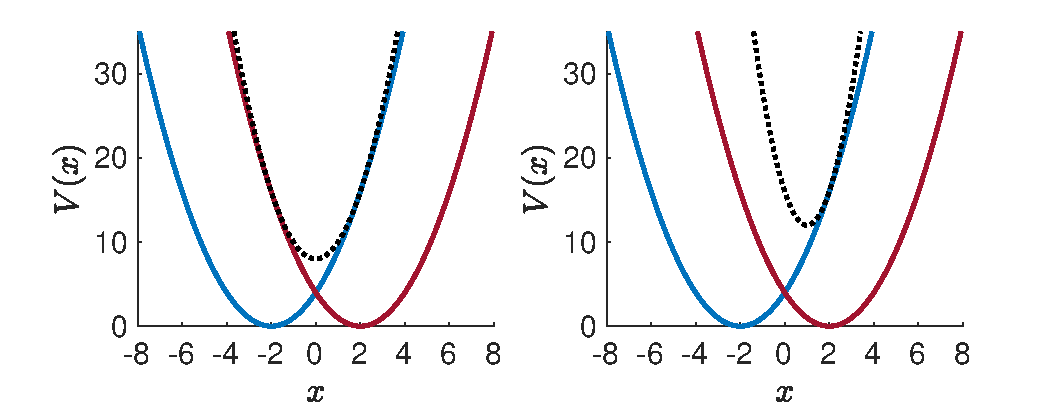
\includegraphics[width=11cm]{figures/ch3/gafos_benus_blending_examples.pdf}
\caption[Examples for blending of vowel gestures by linear combination of the potentials corresponding to each vowel in the model of \citet{GafosBenus2006}.]{Examples for blending of vowel gestures by linear combination of the potentials corresponding to each vowel. Solid lines: individual vowel potentials (blue for $V_B(x)$ and red for $V_F(x)$). Dotted line: combined potential $V_B(x) + V_F(x)$. The two panels show cases for different weightings of the potentials. Left: $\alpha = \beta = 1$, right: $\alpha = 1, \beta = 3$.}
\label{fig:gafos_benus_blending_examples}
\end{figure}

The degree of retraction of a front vowel is assessed by the quantity $R$ in this model of vowel gesture blending. In the example in the right panel of Figure \ref{fig:gafos_benus_blending_examples}, the front vowel described through the potential $V_F(x)$ has a target constriction location of $2$, the vowel resulting from blending has a target location of $1$. In this case, $R$, representing the difference between the basic front vowel and the vowel retracted by influence of the back vowel, is $1$.

The choice of a front vowel or back vowel suffix can now be modelled employing a dynamical system with a double-well potential that uses the retraction degree $R$ as a control parameter. In the system, one attractor is associated with the back suffix, the other attractor is associated with the front suffix. Hence, the second part of the vowel harmony model of \citet{GafosBenus2006} is given by the force $F(x)$ and potential $P(x)$ in Equation \ref{eq:gafos_benus_vowel_harmony_force_potential}. These equations are similar to those in the previous sections. Note, however, that the exposition deviates slightly here and integrates the coefficients for the quartic term $x^4$ and the linear term $x$ from \citet[][262, footnote 85]{Benus2005}.\footnote{The graphs of \citet{GafosBenus2006} are also based on the coefficient $0.1$ for $x^4$, the coefficient of the linear term $x$ is simply put differently.} The choice of this coefficient does not change the general quality of the model; it merely locates the attractor in regions around $-2$ and $2$ corresponding to the assumed values for front and back constriction locations.

\begin{equation}
\begin{split}
F(x) = (2-3R) - 0.4 x^3 + x\\
P(x) = -(2-3R)x + 0.1 x^4 - 0.5 x^2
\end{split}
\label{eq:gafos_benus_vowel_harmony_force_potential}
\end{equation}

Figure \ref{fig:gafos_benus_suffix_potential} presents the graph of the potential $P(x)$ for different values of the control parameter $R$. If the degree of retraction of the transparent vowel is high, e.g. $R = 1.2$ or $R = 1.0$, the attractor landscape only predicts one possibility for the choice of the suffix: back. The reverse is true when the retraction is small, e.g. $R = 0.2$ or $R = 0.4$, for which only front suffixes are possible. In between these values, the attractor landscape becomes bistable. In this region of intermediate $R$ values, the suffix choice can vary between front and back due to random fluctuations and the initial state.

\begin{figure}
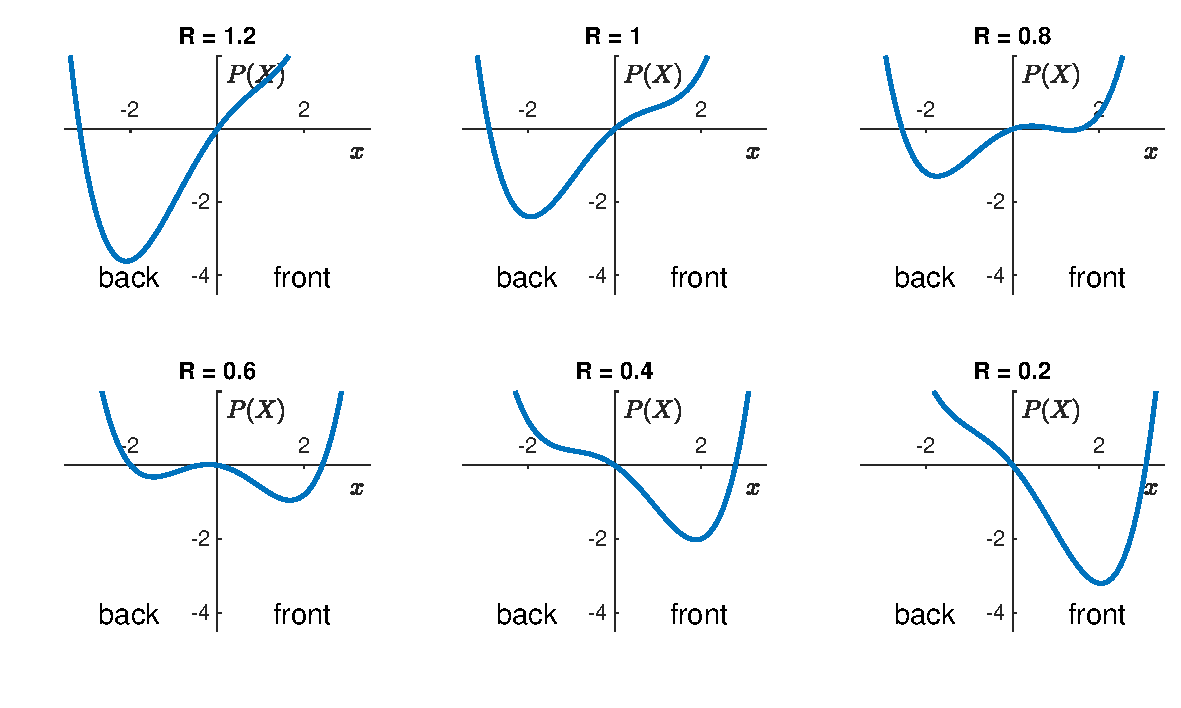
\includegraphics[width=\textwidth]{figures/ch3/gafos_benus_suffix_potential.pdf}
\caption{Suffix choice potential $P(x)$ for different values of the control parameter $R$.}
\label{fig:gafos_benus_suffix_potential}
\end{figure}

The graphs of the potential $P(x)$ shown in Figure \ref{fig:gafos_benus_suffix_potential} illustrate how the scaling of a continuous parameter can lead to categorical changes. Depending on the magnitude of the adjustment of the continuous parameter, only one category remains as the possible output of the system or the system is in principle able to produce two different outcomes. When the system is conceptualised as a stochastic dynamical system, the outcomes of the system depending on the control parameter can be described as statistical distributions. A stochastic system is obtained by the introduction of random fluctuations or noise \citep{Haken1977}, denoted by $\xi_t$ in Equation \ref{eq:gafos_benus_stochastic_system}. $\xi_t$ is conceptualised here as Gaussian white noise with a scaling factor $q$ that determines the strength of the noise \citep{GafosBenus2006}. These statistical distributions of the system's outcome are modulated as a result of the relative stabilities of the attractors. In other words, in the region of bistability, a deeper attractor in the potential is more resistant to random fluctuations than a shallower attractor, it takes more noise to move the system out of the attractor basin. The system is thus more likely to end up in this deeper, more stable attractor.

\begin{equation}
\begin{split}
\dot{x} = F(x) + \text{Noise} = \frac{-dV(x)}{dx} + \xi_t\\
\end{split}
\label{eq:gafos_benus_stochastic_system}
\end{equation}

A description of the distributional patterns of a stochastic system can be obtained in two ways: either analytically by finding a stationary solution to the \emph{Fokker-Planck} equation \citep{Haken1977, FreidlinWentzell1984} or by computational simulation of the system with noise \citep{GafosBenus2006}. The solution to the Fokker-Planck equation is used to compute a probability density distribution. Figure \ref{fig:gafos_benus_probabilities} presents probability distributions obtained in this way for the potential $P(x)$ and the same $R$ values as in Figure \ref{fig:gafos_benus_suffix_potential}.

\begin{figure}
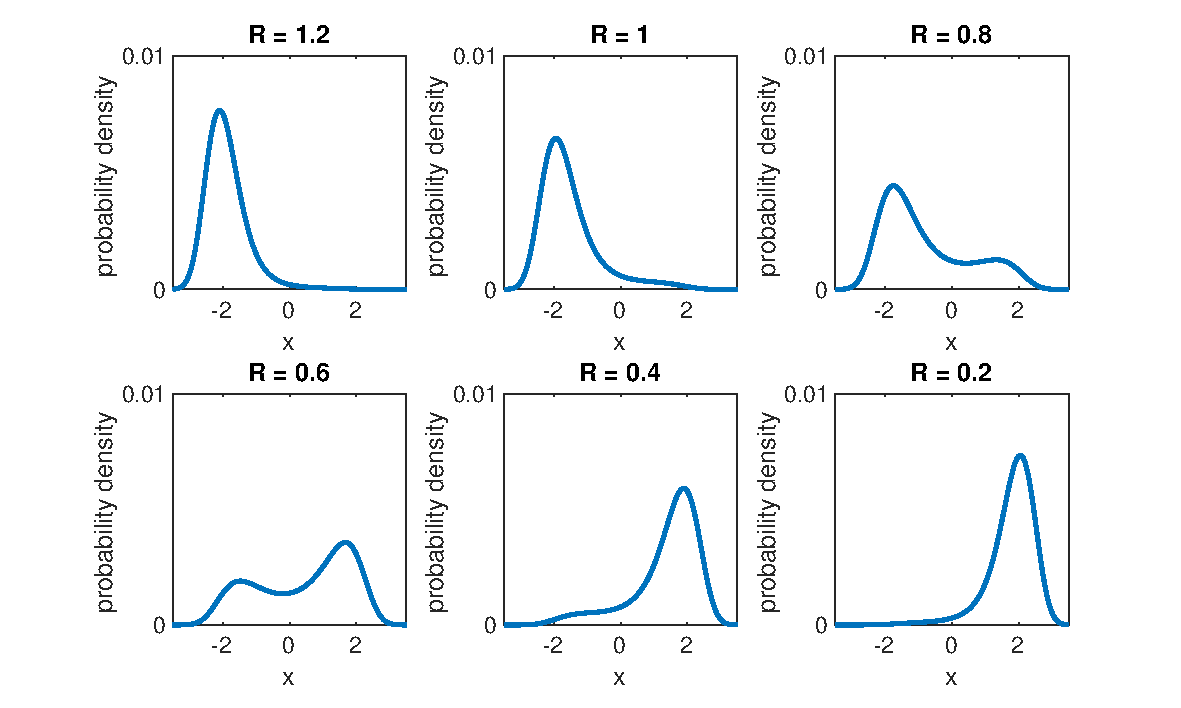
\includegraphics[width=\textwidth]{figures/ch3/gafos_benus_probabilities.pdf}
\caption{Probability density distributions corresponding to the stochastic version of the system described by the potential $P(x)$ for different values of the control parameter $R$.}
\label{fig:gafos_benus_probabilities}
\end{figure}

The simulation of the stochastic system can be carried out by solving the differential equation as described above in Section \ref{sec:diff_equations}. During each time step, noise from a Gaussian distribution is added. After a fixed number of steps, the simulation is finished and the solution is recorded. This procedure is repeated for a number of times in order to obtain a distribution of final solutions. For the solutions shown in the histograms of Figure \ref{fig:gafos_benus_simulation}, the simulation was run for 5000 time steps and repeated to obtain 5000 solutions.\footnote{The simulation is based on the code accompanying \citet{Gafos2006}.} Again, the same values for $R$ as before are chosen in these plots. The outcome of the simulation reproduces the probability density functions shown in the previous figure.

\begin{figure}
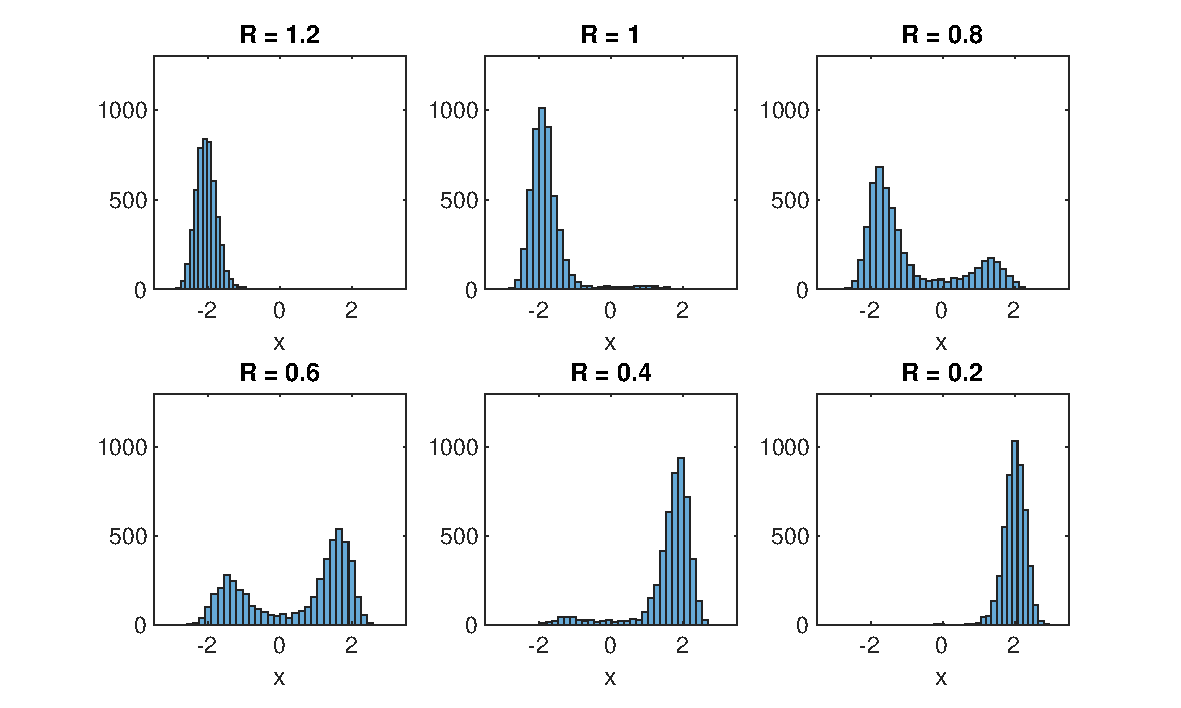
\includegraphics[width=\textwidth]{figures/ch3/gafos_benus_simulation.pdf}
\caption{Simulation results for different values of the control parameter $R$ in the system given by the potential $P(x)$.}
\label{fig:gafos_benus_simulation}
\end{figure}

The concept of the stochastic dynamical system plays a major role for the modelling approach presented in the second part of this book. It makes it possible to leverage the differences in stability of the attractors when multiple attractors are present. This section is completed by taking up the metaphor of a ball rolling in the attractor landscape and adding the notion of noise or random fluctuations to it. Imagine that the ball's trajectory is perturbed by tiny strokes. Sometimes these strokes are stronger, sometimes they are weaker. It fits our intuition well that it takes a stronger stroke to push the ball out of an attractor basin if it is deeper, i.e. more stable, compared to a shallower attractor basin.

\medskip\noindent \textit{Code used in this section: gafos\_benus\_vowel\_harmony.m}

\section{Summary}
This chapter has presented an overview on dynamical systems and their application in the science of language and speech. It has touched upon the fundamental concepts of attractors and multi-stability, and outlined how dynamical systems can be used together with simulation techniques to investigate their predictions in more detail. The most important point to take away from this chapter is that dynamical systems have proven to be suited in reconciling categorical and continuous phenomena in an integrated view and thus provide a toolbox to gain insights into the relation of phonetics and phonology.
